\documentclass[twoside,fontsize=12pt,titlepage]{scrbook}

% * Packages
\usepackage[utf8]{inputenc}
% \usepackage{cite}
\usepackage{graphicx}
\usepackage{eso-pic}
\usepackage[hidelinks]{hyperref}
\usepackage{natbib}
\bibliographystyle{apalike}
\usepackage{color, soul}
\usepackage{xcolor}
\usepackage{pdfpages}
\usepackage{ebgaramond}

\usepackage{gensymb}
\usepackage{makecell}
\usepackage{booktabs}
% \usepackage{tabularx}

% glossary
\usepackage[xindy]{glossaries} 
\newglossaryentry{domain-knowledge}{%
  name={domain knowledge},%
  description={valid knowledge used to refer to an area of human endeavour, an autonomous computer activity, or other specialized discipline}}

\newacronym[description={(Environmental Noise Directive) \emph{DIRECTIVE 2002/49/EC OF THE EUROPEAN PARLIAMENT AND OF THE COUNCIL of 25 June 2002 relating to the assessment and management of environmental noise}. Policy directive within the EU setting out priorities and requirements of member nations for ensuring health and environmental protection as it relates to noise. Incorporates requirements for agglomerations to produce noise maps and identify and preserve quiet areas.}]{end}{END}{Environmental Noise Directive}

\newglossaryentry{isopl}{name={ISOPleasant},description={The value along the primary pleasantness dimension of the soundscape circumplex, calculated via a trigonometric projection of the other \gls{paq}s, as defined in \citet{ISO12913_3_2019IOS}}}

\newglossaryentry{isoev}{name={ISOEventful},description={The value along the primary eventfulness dimension of the soundscape circumplex, calculated via a trigonometric projection of the other \gls{paq}s, as defined in \citet{ISO12913_3_2019IOS}}}

% Psychoacoustic features
%TODO: Write descriptions of psychoacoustic features
\newglossaryentry{laeq}{name={$L_{Aeq}$},description={}}
\newglossaryentry{n5}{name={$N_{5}$},description={Psychoacoustic Loudness}}
\newglossaryentry{s}{name={$S$},description={Psychoacoustic Sharpness}}
\newglossaryentry{r}{name={$R$},description={Psychoacoustic Roughness}}
\newglossaryentry{iu}{name={$I$},description={Impulsiveness}}
\newglossaryentry{fs}{name={$FS$},description={Fluctuation Strength}}
\newglossaryentry{tu}{name={$T$},description={Tonality}}
\newglossaryentry{pa}{name={$PA$},description={Zwicker Psychoacoustic Annoyance}}
\newglossaryentry{la10la90}{name={$L_{A10}-L_{A90}$},description={}}
\newglossaryentry{la10}{name={$L_{A10}$},description={}}
\newglossaryentry{la90}{name={$L_{A90}$},description={}}

\newglossaryentry{lcla}{name={$L_{Ceq}-L_{Aeq}$},description={}}
\newglossaryentry{ra}{name={$RA$},description={Relative Approach}}

\newglossaryentry{environmental-unit}{
  name={environmental unit},
  description={An area within a public space in which environmental factors are consistent and which is typically perceived to constitute a single distinct area.}
}


\newacronym{ssid}{SSID}{Soundscape Indices}
\newacronym{satp}{SATP}{Soundscape Attributes Translation Project}
\newacronym{isd}{ISD}{International Soundscape Database}
\newacronym{wsp}{WSP}{World Soundscape Project}
\newacronym{iso}{ISO}{International Organization for Standardization}
\newacronym{covid19}{COVID-19}{Coronavirus disease of 2019}
\newacronym{slm}{SLM}{Sound Level Meter}
\newacronym{amb}{AMB}{Ambisonic recording}
\newacronym{bin}{BIN}{Binaural}
\newacronym{pic}{PIC}{Site pictures}
\newacronym{vid}{VID}{360\degree Video}
\newacronym{env}{ENV}{Environmental factors}
\newacronym{que}{QUE}{Questionnaires}
\newacronym{ssqp}{SSQP}{Swedish Soundscape Quality Protocol}
\newacronym{paq}{PAQ}{Perceived Affective Quality}
\newacronym{who5}{WHO-5}{WHO-5 Well-being Index}
\newacronym{vr}{VR}{Virtual Reality}
\newacronym{aic}{AIC}{Akaike Information Criterion}
\newacronym{vif}{VIF}{Variance Inflation Factor}
\newacronym{mae}{MAE}{Mean Absolute Error}
\newacronym{wasn}{WASN}{Wireless Acoustic Sensor Network}
\newacronym{rtn}{RTN}{Road Traffic Noise}
\newacronym{ane}{ANE}{Anomalous Noise Event}
\newacronym{complx}{COMPLX}{complex}
\newacronym{mushra}{MUSHRA}{MUlti Stimulus test with Hidden Reference and Anchor}
\newacronym{mlm}{MLM}{Multi-Level Model}
\newacronym[]{pca}{PCA}{Principal Components Analysis}
\newacronym{lmer}{LMER}{Linear Mixed-Effects Regression}
\newacronym{anova}{ANOVA}{ANalysis Of VAriance}
\newacronym{sns}{SNS}{Sympathetic Nervous System}
\newacronym{psns}{PSNS}{Parasympathetic Nervous System}
\newacronym{ans}{ANS}{Auditory Nervous System}
\newacronym{pns}{PNS}{Peripheral Nervous System}
\newacronym{art}{ART}{Attention Restoration Theory}
\newacronym[]{cns}{CNS}{Central Nervous System}
\newacronym[]{sem}{SEM}{Structural Equation Modelling}
\newacronym[]{ci}{CI}{confidence interval}
\newacronym[]{icc}{ICC}{intraclass correlation coefficient}
\newacronym[]{foi}{FOI}{features of interest}
\makeglossaries

% markup commands
\newcommand{\remark}[3]{%
    {\colorbox{#2}{\sffamily\scriptsize\bfseries\textcolor{white}{#1}}}
    {\sffamily\small\itshape\textcolor{#2}{#3}}
}
\newcommand{\misc}[1]{\remark{misc}{green}{#1}}
\newcommand{\draft}[1]{\remark{draft}{blue}{#1}}
\newcommand{\error}[1]{\remark{err}{red}{#1}}
\newcommand{\proof}[1]{\remark{proof}{orange}{#1}}
\newcommand{\cit}[1]{\remark{cit}{brown}{#1}}

% * Formatting
% Margins at the binding edge must not be less than 40mm (1.5 inches) and other margins not less than 20mm (0.75 inches).
% Double or one-and-a-half spacing should be used in typescripts except for indented quotations or footnotes where single spacing may be used.
\usepackage[a4paper,margin=20mm, bindingoffset=20mm]{geometry}
\usepackage[onehalfspacing]{setspace}
\AddToShipoutPicture*
{%
\put(0,730)% the specific point of the page with coordinates (x=100,y=100)
{
\includegraphics[scale=1]{Figures/UCL header.png}}%
}

%%%%%%%%%%%%%%%%%%%%%%%%%%%%%%%%%%%%%%%%%%%%%%%%%%%%%%%%%%%%%%%%%%%%%%%%%%%%%%%%%%%%%%%%%%%%%%%%%%

\begin{document}

\newgeometry{margin=20mm, bindingoffset=0mm}
\begin{titlepage}
      % The title page must bear the following:
      % - the officially-approved title of the thesis
      % - the candidates full name as registered
      % - the institution name 'UCL'
      % - the degree for which the thesis is submitted
      \AddToShipoutPicture*{}
      \begin{center}
            \vspace*{3cm}

            \Huge
            \textbf{Predictive Modelling of Complex Urban Soundscapes}

            \vspace{0.5cm}
            \LARGE
            % Thesis Subtitle
            Multi-level Regression and Deep Learning Approaches

            \vspace{1.5cm}

            \textbf{Andrew James Mitchell}

            \vfill
            A thesis presented for the degree of\\
            Doctor of Philosophy\\
            \rule[-.5cm]{0.5\textwidth}{1pt}

            \vspace{1.5cm}

            \Large
            Institute for Environmental Design \& Engineering\\
            University College London (UCL)\\
            \today

            \vspace{1cm}

            Principal Supervisor: Prof. Jian Kang\\
            Co-Supervisor: Dr. Phil Symonds

      \end{center}
\end{titlepage}


\restoregeometry

%%%%%%%%%%%%%%%%%%%%%%%%%%%%%%%%%%%%%%%%%%%%%%%%%%%%%%%%%%%%%%%%%%%%%%%%%%%%%%%%%%%%%%%%%%%%%%%%%%

\chapter*{Declaration}
% The title page should be followed by a signed declaration that the work presented in the thesis is the candidate's own:
I, Andrew Mitchell, confirm that the work presented in this thesis is my own. Where information has been derived from other sources, I confirm that this has been indicated in the thesis.

\chapter*{Abstract}
% The signed declaration should be followed by an abstract consisting of no more than 300 words


\chapter*{Acknowledgements}
This research was funded by the European Research Council.

People to thank:
\begin{itemize}
      \item Dr Francesco Aletta
      \item Prof Jian Kang
      \item Dr Tin Oberman
      \item Dr Phil Symonds
      \item Ms Mercede Erfanian
      \item Ms Magdalena Kachlicka
      \item Mr Matteo Lionello
      \item Friends: Nicole Watson, Nick Wilson, Valentina
\end{itemize}

\chapter*{List of Studies}

This doctoral thesis is based on the following studies:

\paragraph*{}
\textbf{Mitchell, A.}, Oberman, T., Aletta, F., Erfanian, M., Kachlicka, M., Lionello, M., \& Kang, J. (2020) The Soundscape Indices (SSID) Protocol: A Method for Urban Soundscape Surveys -- Questionnaires with Acoustical and Contextual Information. \emph{Applied Sciences, 10} (7), 2397. \url{https://doi.org/10.3390/app10072397}

\paragraph*{}
Erfanian, M., Mitchell, A. J., Kang, J., \& Aletta, F. (2019). The Psychophysiological Implications of Soundscape: A Systematic Review of Empirical Literature and a Research Agenda. \emph{International Journal of Environmental Research and Public Health, 16(19)}, 3533. https://doi.org/10.3390/ijerph16193533

\paragraph*{}
Erfanian, M., \textbf{Mitchell, A.}, Aletta, F., \& Kang, J. (2020). Psychological Well-being and Demographic Factors can Mediate Soundscape Pleasantness and Eventfulness: A large sample study. \emph{Environmental Psychology}.

\paragraph*{}
Orga, F., \textbf{Mitchell, A.}, Freixes, M., Aletta, F., Alsina-Pagès, R. M., \& Foraster, M. (2021). Multilevel Annoyance Modelling of Short Environmental Sound Recordings. \emph{Sustainability, 13}(11), Article 11. \url{https://doi.org/10.3390/su13115779}

\paragraph*{}
\textbf{Mitchell, A.}, Oberman, T., Kachlicka, M., Aletta, F., Lionello, M., Erfanian, M., \& Kang, J. (2021). Investigating Urban Soundscapees of the COVID-19 Lockdown: A predictive soundscape modelling approach. \emph{JASA}.

\paragraph*{}
\textbf{Mitchell, A.}, Soelitsyo, C., Erfanian, M., Xue, J-H., Oberman, T., Kang, J., \& Aletta, F. (2021). A Temporal Convolutional Neural Network for Multi-label Sound Recognition and Annoyance Detection of Complex Soundscapes. \emph{IEEE}.

\paragraph*{}
\textbf{Mitchell, A.}, Aletta, F., Chalabi, Z., \& Kang, J. (2021). From Deterministic to Probabilistic Soundscapes: A critical tour around the soundscape circumplex. \emph{JASA-EL}.

\paragraph*{}
Kang, J., Aletta, F., Oberman, T., \textbf{Mitchell, A}., Erfanian, M., Tong, H., Torresin, S., Xu, C., Yang, T. (2021). Supportive Soundscapes are Crucial for Sustainable Cities and Communities. \emph{Nature Sustainability}.



%%%%%%%%%%%%%%%%%%%%%%%%%%%%%%%%%%%%%%%%%%%%%%%%%%%%%%%%%%%%%%%%%%%%%%%%%%%%%%%%%%%%%%%%%%%

\newpage
The following studies are related works which influenced this thesis and were completed as part of the same work but have not been included as key components:

\paragraph*{}Erfanian, M., \textbf{Mitchell, A. J.}, Kang, J., \& Aletta, F. (2019). The Psychophysiological Implications of Soundscape: A Systematic Review of Empirical Literature and a Research Agenda. \emph{International Journal of Environmental Research and Public Health, 16(19)}, 3533. \url{https://doi.org/10.3390/ijerph16193533}

\paragraph*{}Lionello, M., Aletta, F., \textbf{Mitchell, A.}, \& Kang, J. (2020). Introducing a Method for Intervals Correction on Multiple Likert Scales: A Case Study on an Urban Soundscape Data Collection Instrument. \emph{frontiers in Psychology}.

\paragraph*{}Aletta, F., Oberman, T., \textbf{Mitchell, A.}, Tong, H., \& Kang, J. (2020). Assessing the changing urban sound environment during the COVID-19 lockdown period using short-term acoustic measurements. \emph{Noise Mapping}.

% \paragraph*{}Tong, H., Aletta, F., \textbf{Mitchell, A.}, Oberman, T., \& Kang, J. (2021). Increases in noise complaints during the COVID-19 lockdown in Spring 2020: A case study in Greater London, UK. \emph{Science of the Total Environment}.



\chapter*{Impact Statement}
% The abstract should be followed by an impact statement consisting of no more than 500 words.
The statement should describe, in no more than 500 words, how the expertise, knowledge, analysis, discovery or insight presented in your thesis could be put to a beneficial use. Consider benefits from \textbf{inside} and \textbf{outside} academia and the ways in which these benefits could be brought about.

\chapter*{COVID-19 Statement}

In March of 2020, 18 months into the development of this thesis, the COVID-19 pandemic hit the UK, forcing it into lockdowns which would continue for over a year. Solely by good fortune and a tendency to speed ahead with too-little thought, the primary data collection had fortunately been completed prior to the first lockdown. However, this work was impacted in three ways:

\begin{enumerate}
      \item Further in-situ data collection could not be completed, reducing the range of soundscape types we could include;
      \item The unprecedented and stressful world of the pandemic had a significant mental health and social impact, the effects of which cannot be quantified, nor overstated;
      \item In response to the unique scientific opportunity of a world-wide transportation and social lockdown, new, unplanned studies were carried out.
\end{enumerate}

In particular, this final point has had an impact on the structure and content of this thesis. Certain aspects of the research, in particular the model development and building, were accelerated and put into practice to investigate the impacts of the COVID lockdowns, before being returned to and further developed. The initial research plan would have followed a more logical path of nailing down the model development first, then moving on to a first implementation. In addition, new work was added to this thesis which may appear incongruous or unrelated, but represents a great deal of necessary work which further informed the key strains of the thesis.



%%%%%%%%%%%%%%%%%%%%%%%%%%%%%%%%%%%%%%%%%%%%%%%%%%%%%%%%%%%%%%%%%%%%%%%%%%%%%%%%%%%%%%%%%%%%%%%%%%

\tableofcontents
% In each copy of the thesis the abstract should be followed by a full table of contents (including any material not bound in) and a list of tables, photographs and any other materials.

% \listoffigures
% \listoftables

\chapter{Introduction}
\label{ch:intro}

\section{Research Summary}
Urban noise pollution affects 80 million EU citizens with substantial impacts on public health which are not well addressed by conventional noise control methods. Traditional noise control methods have typically limited their focus to the reduction of unwanted noise, ignoring the potential benefits of increasing positive sounds and remaining restricted by practical limitations of noise reduction. Modern approaches to achieve improved health outcomes and public satisfaction aim to incorporate a person's perception of an acoustic environment, an approach known as 'Soundscape'.

Soundscape studies strive to understand the perception of a sound environment, in context, including acoustic, (non-acoustic) environmental, contextual, and personal factors. These factors combine together to form a person's soundscape in complex interacting ways \citep{Berglund2006Tool}. In order to predict how people would perceive an acoustic environment, it is essential to identify the underlying acoustic and non-acoustic properties of soundscape.

% From: Upgrade report
When attempting to apply soundscape in practical applications in the built environment, it is immediately apparent that a predictive model of the users' perceptual response to the acoustic environment is necessary. Whether to determine the impact of a design change, or to integrate a large scale data at neighbourhood and city levels, a mathematical model of the interacting factors will form a vital component of the implementation of the soundscape approach. This work is intended to identify methods for incorporating contextual and objective information into a useable and interpretable predictive model of urban soundscapes. In order to achieve this, a protocol for collecting the multi-level, multi-factor perceptual assessment data has been developed and implemented, resulting in a large soundscape database. Several avenues of investigation are then drawn from the database and addressed throughout this thesis. The primary research questions are:

% TODO: Try to move this to the end of the introduction.
\begin{enumerate}
  \item What are the primary acoustic features involved in soundscape formation and what are the driving interactions between acoustic features and soundscape assessment?
  \item How does the sound source composition in a complex sound environment mediate this interaction and how can this effect be simplified and modelled?
  \item How can the multiple levels of soundscape formation be simplified and integrated into a cohesive predictive model, and what interpretations about the cross-effects of these levels can be drawn from the model?
  \item In what ways and to what extent can predictive soundscape modelling be applied to address future urban design challenges? How can these methods best be integrated into policy, design, noise mapping, and engineering practice?
\end{enumerate}

Towards answering these questions, the results of five %TODO: check this number at the end.
peer-reviewed studies are presented. These studies represent a series of work to 

\begin{enumerate}
  \item Advance the conceptual development and practice of soundscape studies
  \item Develop a transparent and useful method of predicting soundscape assessments
  \item Investigate the various components which influence soundscape perception, including personal factors like psychological well-being, acoustical factors, and sound source specifics and to integrate these components into the predictive modelling methods.
\end{enumerate}

\section{The SSID Project}
The \gls{ssid} Project is a five-year, multi-disciplinary project funded by a Horizon 2020 European Research Council grant (no. 740696).

\subsection{Project collaborators}

\subsection{Motivation for the SSID Project}

\section{Research Aims}

\section{Soundscape Indices and Metrics}

\section{General Aim}


%%%%%%%%%%%%%%%%%%%%%%%%%%%%%%%%%%%%%%%%%%%%%%%%%%%%%%%%%%%%%%%%%%%%%%%%%%%%%%%%%%%%%%%%%%%%%%%%%%%%

\chapter{Literature Review}
\label{ch:lit}

\section{Impact of Urban Noise on Health and Wellbeing}

\cit{Environmental noise in Europe 2020}

\hl{Give a full formal background to why noise control is important for public health}.
% https://www.euro.who.int/__data/assets/pdf_file/0008/383921/noise-guidelines-eng.pdf?ua=1

\section{Current Methods of Assessing and Addressing Urban Noise}

The approach to a practical predictive soundscape model arrived at within this thesis is heavily based on past environmental acoustics approaches. I will therefore begin with a brief summary of these past approaches.

\subsection{Acoustical Parameters}

\subsection{ISO Environmental Acoustics Standards}
\hl{ISO 1996-1, esp sections on annoyance, e.g. Annex F, G, H}

\subsection{EU Noise Mapping}

\cit{Environmental noise in Europe 2020}

\subsection{Shortcomings}


\section{Soundscape Studies}

\subsection{Soundscape Descriptors and Indices}

\subsection{World Soundscape Project}

\subsection{Swedish Soundscape Quality Protocol}


\subsection{Demographic differences}
Several studies have attempted to study the degree to which personal and demographic factors influence a person's soundscape perception. In some conceptions \cit{Kou2020effects} % CITE add Erfanian 2020
these personal factors are classed as 'contextual' soundscape indicators - features which influence or, in a modelling context, be used as independent variables to predict the value of a soundscape descriptor. The personal factors help to create a personal soundscape interpretation model which is individual to each person.

In this way, a person's individual state-of-mind, ethnic identity, educational background, gender identity, etc. form a pseudo-deterministic framework %! what a load of crap
through which the physical inputs from their environment are filtered. Clearly, many of these personal factors could never be measured and even those which are measurable will have wide ranges of legitimate effects, however estimating the degree and type of effect they may have can both help us better predict individual soundscape assessments and understand how group identities influence sound perception.

%TODO: Need to include earlier, more foundational studies into demographic factors

\paragraph*{Section on Erfanian et al. 2020, Psychological Well-being}

\paragraph*{Low-income and minority evidence} % FIXME I think this section will need to be heavily revised for phrasing and content. I'm not happy with how I'm discussing under-represented groups.
A consistent limitation of soundscape studies investigating the influence of personal factors is a sampling bias towards majority ethnicities (typically White British for UK studies and ethnic Chinese for Chinese studies) and middle-class and highly educated groups. % CITE Hoo boy citation definitely needed
This results in not only incomplete information about how demographics influence soundscape perception, but also represents a systemic under-representation of certain environments. While it may be unclear to what extent ethnicity and social class internally influence a person's perception, it is clear that these groups are exposed to different sound environments % NOTE: socio-economic studies - Huan 2019? Jian ~2015?, Environmental noise in Europe 2020

and therefore studies which do not include under-represented groups are also by definition not including those sound environments which those groups inhabit.

A recent study by \cit{Kou2020effects} was successful in making inroads in these under-represented environments by studying the Humboldt Park neighbourhood in Chicago, USA. Their study included
% TODO: Finish summarising results from Kou2020


\section{Approaches to Soundscape in Engineering}

From this literature review, some conclusions about current approaches to incorporating the concept of "soundscape" into practical engineering and architectural design have been identified.

\subsection{The Quiet Areas approach}

This approach maintains a focus on "identifying and preserving quiet areas" \cit{Environmental noise in Europe 2020} following the imperative given in the Environmental Noise Directive \cit{END}. This approach is mostly rooted in a noise mindset, although the methods employed for identifying quiet areas varies across countries within the EEA. Background sound levels seem to play an important role in identifying quiet areas, in particular when attempting to

%TODO Continue adding from Remarkable notes

\section{Existing Predictive Models}

Contrary to the hopes expressed by \citet{Aletta2014Towards}, that "ideally there should be one acoustic indicator per dimension", the evidence from subsequent investigations and modelling attempts \citep{Lionello2020systematic} indicates this to be unlikely. There appears to be no reason we should think the perceptual dimensions should be reduced to a single acoustic indicator. The dimensions of soundscape represent complex perceptual concepts which we should expect to be composed of a multi-factor interaction between the input features. This necessary complexity  highlights the need for a more sophisticated machine learning approach in order to handle and interpret the interactions between the many input features which contribute to the formation of a soundscape perception.
\citep{Aletta2016Soundscape}

\citep{Lionello2020systematic}

\subsection{Models based on non-acoustic data sources}

\citep{Verma2020Predicting}, \citep{Gasco2020Social}



%%%%%%%%%%%%%%%%%%%%%%%%%%%%%%%%%%%%%%%%%%%%%%%%%%%%%%%%%%%%%%%%%%%%%%%%%%%%%%%%%%%%%%%%%%%%%%%%%%%%
% \chapter{Methods}
\label{chap:methods}

%%%%%%%%%%%%%%%%%%%%%%%%%%%%%
%FIXME: Find a better spot for this
The ability to predict the likely soundscape assessment of a space is crucial to implementing the soundscape concept in practical design. Current methods of assessing soundscapes are generally limited to a post-hoc assessment of the existing environment, where users of the space in question are surveyed regarding their experience of the acoustic environment \citep{Engel2018Review, Zhang2018Effect}. While this approach has proved useful in identifying the impacts of an existing environment, designers require the ability to predict how a change or proposed design will impact the soundscape of the space. To this end, a model that is built upon measurable or estimate-able quantities of the environment would represent a leap forward in the ability to design soundscapes.

\section{Questionnaires}

 The full protocol developed for this thesis is outlined in Chapter \ref{chap:protocol}. The development and presentation of this protocol involved a substantial development and testing phase, and represents a novel advancement in soundscape survey methodology. Therefore it was submitted and published as a peer-reviewed journal article in MDPI Applied Sciences as \citet{Mitchell2020Soundscape} and is presented as a stand-alone chapter within this thesis.

 \subsection{Likert Responses}

 \subsection{Circumplex Projection}

\section{Psychoacoustics and Auditory Perception}

 \subsection{Psychoacoustic Parameters}

   \subsubsection{Loudness}
   \emph{Zwicker and Fastl, Chap 8, see Mendeley notes and python-acoustics development notes.}
 \subsection{Feature Selection}

\section{Machine Learning and Regression Techniques}

 \subsection{Feature Selection}
   \subsubsection{Mutual Information}
   \draft{It appears that mutual information is related to the Bayes formula. I still need to read more into this, but it appears based on relative and overlapping probability distributions between the variables in question.}
   \paragraph*{From scholarpedia:}
   % http://www.scholarpedia.org/article/Mutual_information
   \draft{Based on entropy, where the uncertainty about a variable can be expressed as "the number of yes/no questions it takes to guess a random variable, given knowledge of the underlying distribution and taking the optimal question-asking strategy". "The mutual information is therefore the \emph{reduction} in uncertainty about variable $X$, or the expected reduction in the number of yes/no questions needed to guess $X$ after observing $Y$.". }

   \draft{"Mutual Information is just one way among many of measuring how related two variables are. However, it is a measure ideally suited for analyzing communication channels. Abstractly, a communication channel can be visualized as a transmission medium which receives an input $x$ and produces an output $y$. If the channel is \emph{noiseless}, the output will be equal to the input. However, in general, the transmission medium is noisy and an input $x$ is converted to an output $y$ with probability $P_{Y|X}(y|x)$. }
   \misc{This seems very useful for my conception of sound perception / auditory processing, where the perception system is a noisy communication channel.}

   \subsubsection{Conditional Mutual Information}
   The Mutual Information between two variables, given another variable as a control.

 \subsection{Clustering Analysis}
   \paragraph{K-means}
   \paragraph{nbclust}

 \subsection{Modelling Likert-type Data}

   \subsubsection{Multiple Linear Regression}

   \subsubsection{Ordinal Logistic Regression}

   \subsubsection{Multi-output Regression}

 \subsection{Multi-level Models}

 \subsection{Bayesian Regression}


\chapter{\label{pap:prot}Protocol: The Soundscape Indices (SSID) Protocol: A Method for Urban Soundscape Surveys -- Questionnaires with Acoustical and Contextual Information}

\section{Background and aims}
Conducting urban soundscape studies on a scale large enough to form a machine learning dataset presents a unique challenge. The standardised methods of conducting soundscape surveys \citep{ISO12913_2_2018IOS} are labour-intensive, time-consuming, and provide limited information about the acoustical and environmental context.

\subsection*{Result and conclusions}

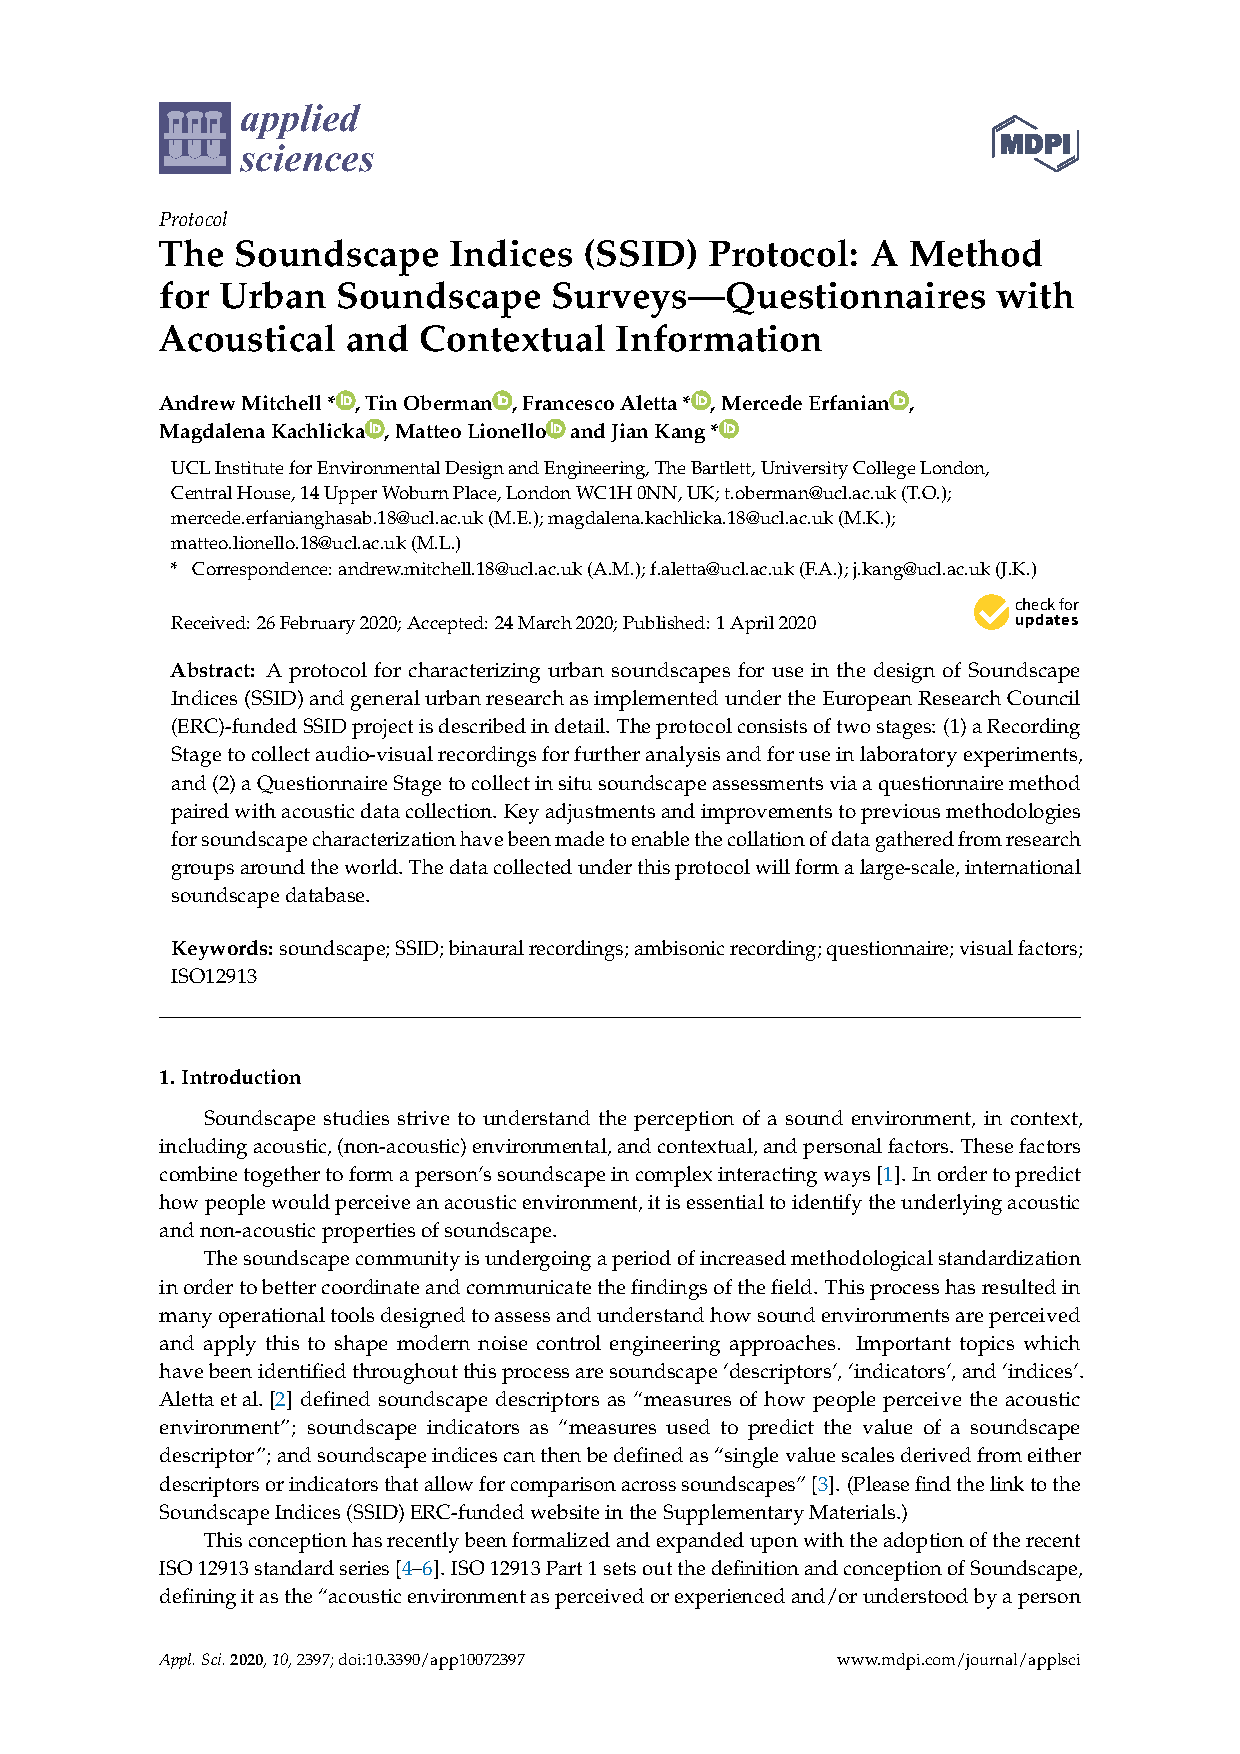
\includepdf[pages={1-16}]{./Papers/Mitchell2020Soundscape.pdf}

%%%%%%%%%%%%%%%%%%%%%%%%%%%%%%%%%%%%%%%%%%%%%%%%%%%%%%%%%%%%%%%%%%%%%%%%%%%%%%%%%%%%%%%%%%%%%%%%%%%%


\section{Study I: Psychological Well-being and Demographic Factors can Mediate Soundscape Pleasantness and Eventfulness: A large sample study}

\subsection*{Background and aims}

\hl{Some summary text here.}

\subsection*{Result and conclusion}

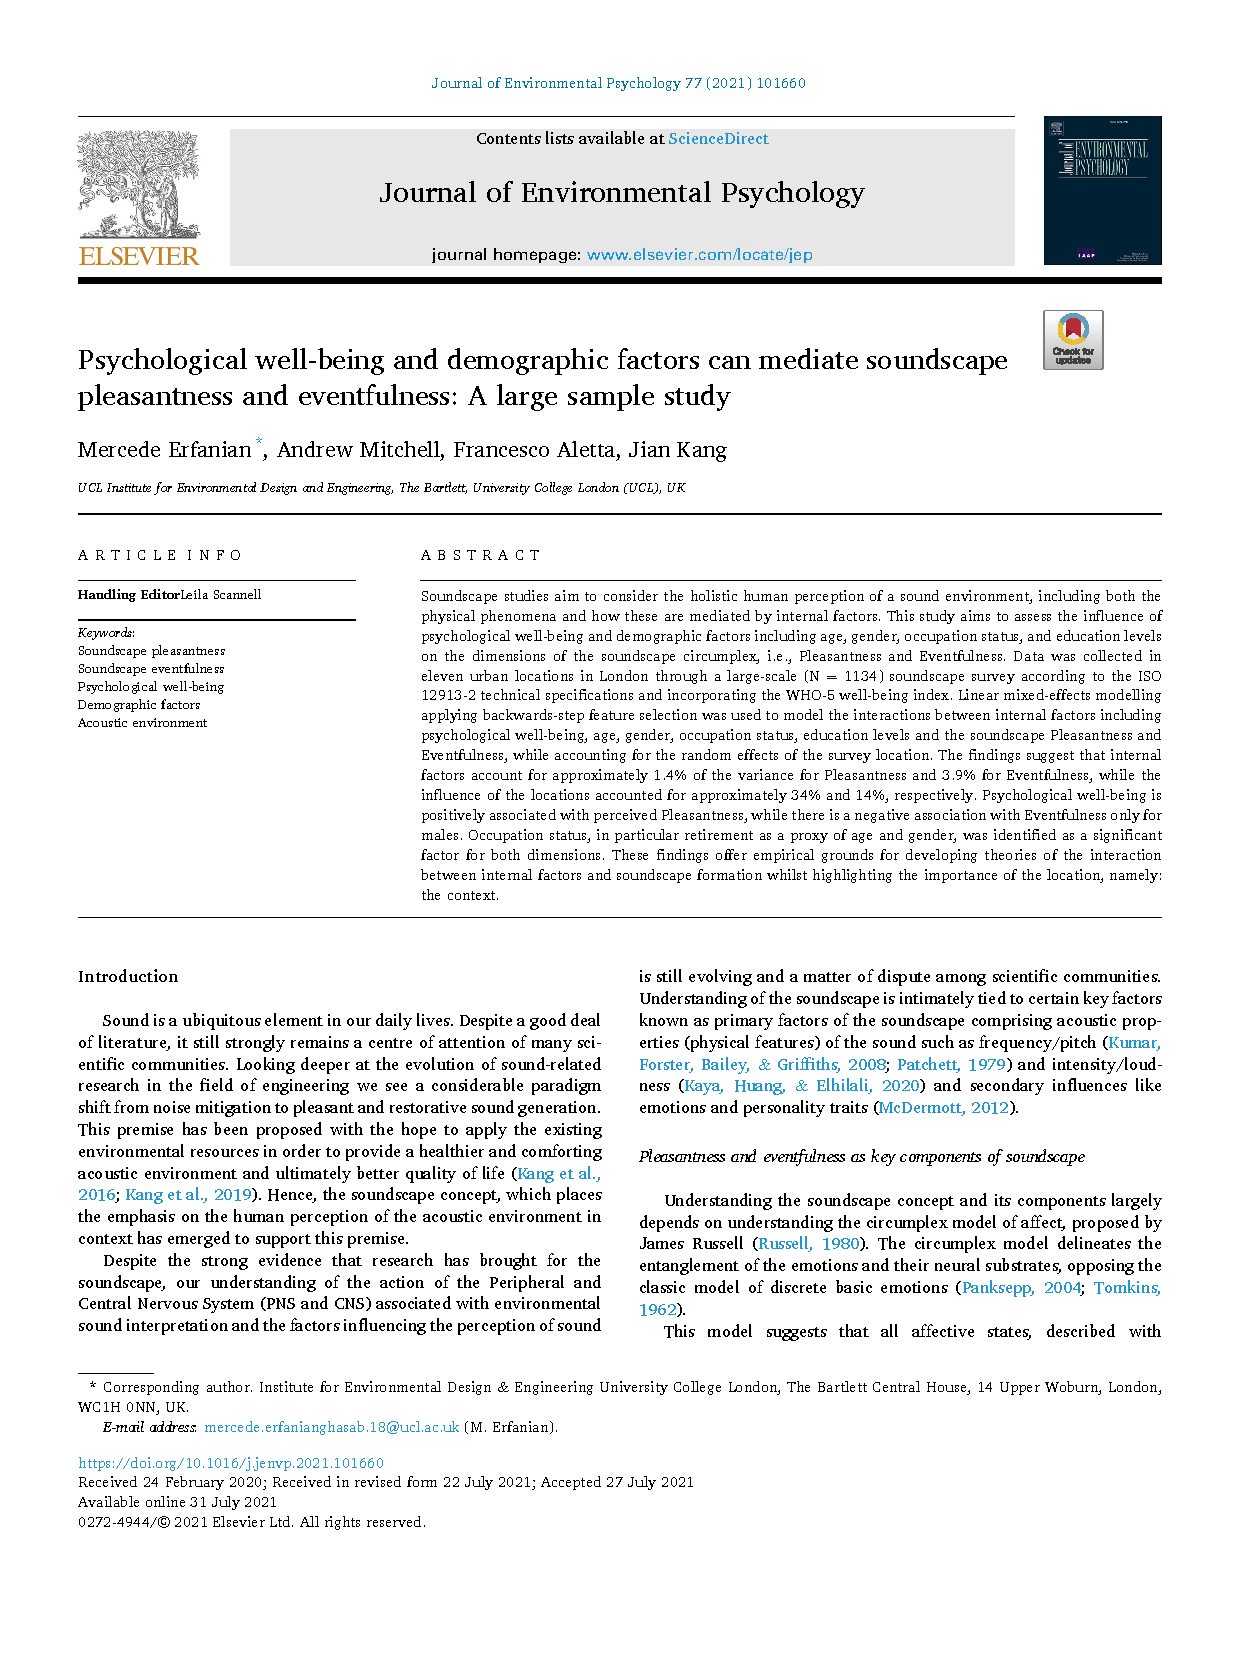
\includepdf[pages={1-8}]{./Papers/Erfanian2021Psychological - Psychological Well Being and Demographic Factors Can Mediate Soundscape Pleasantness and Eventfulness_ a Large Sample Study.pdf}

%%%%%%%%%%%%%%%%%%%%%%%%%%%%%%%%%%%%%%%%%%%%%%%%%%%%%%%%%%%%%%%%%%%%%%%%%%%%%%%%%%%%%%%%%%%%%%%%%%%%

\chapter{Multilevel Annoyance Modelling of Short Environmental Sound Recordings Including Sound Source Information}
\label{ch:mlmann}

\section*{Context}
Published as: Orga, F., \textbf{Mitchell, A.}\footnote{Joint first author}, Freixes, M., Aletta, F., Alsina-Pagès, R. M., \& Foraster, M. (2021). Multilevel Annoyance Modelling of Short Environmental Sound Recordings. \emph{Sustainability, 13}(11), Article 11. \url{https://doi.org/10.3390/su13115779}

%TODO: Need to heavily edit this to rephrase and to re focus on my work
\draft{This chapter will be re-worded and somewhat reorganised to better fit my thinking and to highlight the analysis work. Its focus within the thesis is on the use of sound source information to improve the prediction of annoyance. Right now this is wholesale copied from the published paper.}

\section*{Abstract}

 \draft{The recent development and deployment of Wireless Acoustic Sensor Networks (WASN) present new ways to address urban acoustic challenges in a smart city context. A focus on improving quality of life forms the core of smart-city design paradigms and cannot be limited to simply measuring objective environmental factors, but should also consider the perceptual, psychological, and health impacts on citizens. This study therefore makes use of short (1 - 2.7s) recordings sourced from a WASN in Milan which were grouped into various environmental sound source types and given an annoyance rating via an online survey with $N=100$ participants. A multilevel psychoacoustic model was found to achieve an overall $R^2=0.64$ which incorporates Sharpness as a fixed effect regardless of the sound source type and Roughness, Impulsiveness, and Tonality as random effects whose coefficients vary depending on the sound source. These results present a promising step torward implementing an on-sensor annoyance model which incorporates psychoacoustic features and sound source type, and is ultimately not dependent on sound level.}

\section{Introduction}

 \draft{Noise has been proven to have a wide impact on the social and economic aspects of citizens' lives \citep{Goines2007Noise} and is regarded as one of the primary environmental health issues referenced in the new environmental noise guidelines \citep{Nations2018World}. Over the past few years, several research teams have analysed the causes and the impact of this noise, revealling that it causes more than 48,000 new cases of ischemic heart disease and around 12,000 deaths in Europe each year \citep{Blanes2017Noise}. Furthermore, it leads to chronic high annoyance for more than 22 million people, and sleep disturbance for more than 6.5 million people \citep{Ndrepepa2011Relationship}. One of the main noise sources according to research is road traffic noise \citep{Ouis2001Annoyance}, causing psychological reactions in citizens \citet{Basner2006Aircraft} and even cardiovascular diseases \citep{Ndrepepa2011Relationship}.}

 \draft{Other studies analyse the effects of aircraft noise on sleep \cit{} and learning impairments in children \cit{}. Also, railway noise has proven to cause annoyance due to its huge variety of sounds, e.g. rail breaks, whistles, squeals, and vibrations \cit{ 8, 9}. Most of the literature focuses on sound level measurements and the corresponding annoyance \cit{ 10}, but other acoustical and psychoacoustical characteristics could be taken into account, e.g. loudness or sharpness \cit{ 11}, in order to understand the degree of noise annoyance and identify the characteristics of sounds that may be more detrimental to psychological well-being and consequently for health. Such knowledge is relevant for policy makers and urban planners in order to create healthy environments.}

 \draft{Several tests used in studies to evaluate the effects of environmental noise for citizens \cit{ 12} can be used to design this model. This study uses real-life data and its sound characterisation, thus focusing on noise sensitivity was not the closes approach to the problem. The tests used as a basis in this work have been defined with the purpose of finding new ways of analysing the impact of sound -- usually traffic -- on citizens in urban environments \cit{ 13, 14}, in order to model the annoyance perception \cit{15, 16}.}

 \draft{The perceptual tests were designed to measure the annoyance in people relating to different urban sounds and their characteristics \cit{ 17, 18}, by means of short excerpts of raw acoustic audio obtained from the DYNAMAP project \cit{ 19}. The most representative audio excerpts were selected, using a wide range of sound types (sirens, airplanes, people talking, dogs barking, etc.) \cit{ 20, 21}. However, sound annoyance depends on the acoustic characterisation of each sample, and it is possible to classify the acoustic excerpts depending on their characterisation, which can be the basis to ask participants about their perceptions. The characterisation is based on the psychoacoustic measurements of loudness, sharpness, and others defined by Zwicker \cit{ 11}.}

 % FIXME will need to rewrite this paragraph, not happy with it.
 \draft{The researchers asked more than 100 people to conduct the perceptual tests \cit{18}. Some preliminary results of the three tests conducted were published in \cit{17} in which the relationship between sharpness and annoyance was analysed by means of an A/B test \cit{22}, and later on in \cit{18}, where some of the research questions were formulated. In this study, I aim to determine the parameters that have an effect in the individual annoyance scores. For this reason, a multilevel psychoacoustic model is trained using the results of the MUSHRA \cit{23} test, essentially focused on annoyance evaluation by the participants over several different types of sound, while loudness and sharpness were kept constant. The results show that the differences in annoyance perception between the different demographic groups is not statistically significant and that sharpness is the main predictor for annoyance.}

 The chapter is structured as follows: Section \ref{sec:mod} detailes the state-of-the-art of annoyance modelling by means of subjective data collection. Section \ref{sec:proc} describes the procedure followed in this work, including the dataset and the design of the perceptual test. In section \ref{sec:res} the results obtained from the perception tests are presented and discussed, and the annoyance model is proposed. Section \ref{sec:disc} contains the discussion and, finally, Section \ref{sec:conc} presents the conclusions of the study.

\section{State of the Art of Annoyance Evaluation and Modelling}
 \label{sec:mod}
 In this section I gather a short synthesis of the most relevant contributions of the state-of-the-art on which the design of the tests and the modelling of perceptual annoyance have been based.

 \subsection{Evaluation of Annoyance}
   % FIXME prob need to rewrite this
   \draft{The evaluation of annoyance can be found in literature by means of the objective parameters related to sound and noise \cit{10}. Nevertheless, when the goal is to measure the perception -- the real annoyance experienced by people -- one of the most frequently used methods is to conduct a survey to measure the degree of annoyance produced by different sounds \cit{24, 25,26}. Following the recommendation of the International Committee for the Biological Effects of Noise (ICBEN), this evaluation should be done in a qualitative way, using a verbal scale; this can be translated into \emph{not at all, slightly, moderately, very} and \emph{extremely}, just to give a few examples. Also an 11-point scale -- also from an ICBEN recommendation -- can be used, where in this case, zero corresponds to \emph{not at all} and 10 corresponds to \emph{extremely disturbing}.}

   % FIXME take this paragraph out
   \draft{Furthermore, taking advantage of the experience in soundscape evaluation \cit{27} citizens can be asked about other aspects besides annoyance. To this end a perceptual assessment based on a Likert scale \cit{28} could be used. This scale defines five levels of agreement with a given statement: \emph{Strongly disagree, Disagree, Neither agree nor disagree, Agree} and \emph{Strongly agree}. This scale was used in \cit{17,18} to evaluate several types of noise sources according to a small group of attributes such as \emph{loud, shrill, noisy, disturbing, sharp, exciting, calming} and \emph{pleasant} (see the complete list of adjectives in \cit{27}).}

  Borrowing from the subjective assessment of audio quality, the MUSHRA method has been also used for the evaluation of annoyance in \cit{17, 18}. \gls{mushra} was described and designed by ITU-R under the recommendation ITU-R BS.1534-3 \cit{23}. This recommendation gives guidelines on listening tests and subjective assessment, as well as audio quality (among other applications), assuming that the best way to evaluate audio quality is by means of subjective listening.

   Listening tests can be conducted in a controlled scenario (e.g. in an anechoic chamber) thus allowing the organiser to have control over the setup and experimental design. Nevertheless, this approach is expensive and time consuming. Alternatively, online listening tests have been widely used in the perceptual evaluation of audio quality or speech synthesis systems, even resorting to crowdsourcing strategies \cit{29}. These tests can be run in parallel and anywhere, thereby reducing costs and allowing researchers to reach a wider audience \cit{30}. In addition, these tests have seen increased use in the wake of the \gls{covid19} pandemic and its subsequent lockdowns. The limited access to facilities and equipment restricted how socio-acoustic and laboratory studies could be conducted, leading to the development of new online data collection methods. Recommendations for conducting such studies were given by \draft{the Acoustical Society of America in \cit{that guidance site}}. %TODO: Expand on this bit?

 \subsection{Annoyance Prediction}
   \draft{After the design and execution of the perceptual tests, the resulting evaluation coming from participants are used to generate a model that can predict the annoyance value depending on the type and the parameters of the noise excerpt under study. One of the most representative examples of annoyance modelling is found in \cit{15}, where a model based on the hypothesis that annoyance is primarily determined by the detection of intruding sounds is presented. The model takes into account several measurable elements:}

   \begin{enumerate}
     \item signal-to-noise ratio (SNR);
     \item indoor background level;
     \item the activity conducted by the listener, assuming that in the conducted tests, their main activity is not listening to events.
   \end{enumerate}

   \draft{The model is obtained from the results of a test evaluating annoyance and acoustic data from a field experiment in a natural setting.}

   Another reference model for annoyance prediction is found in \cit{16}, where the authors model and predict road traffic noise annoyance based on:
   \begin{enumerate}
     \item noise perception;
     \item noise exposure levels;
     \item demographics.
   \end{enumerate}

   \draft{The authors apply machine-learning algorithms in order to conduct the prediction and measure error rates, which give them a good trade-off in the prediction of the traffic noise annoyance, with a strong dependence on subjective noise perception and predicted noise exposure levels, assuming that the classical statistical approaches fail in their predictions in terms of accuracy.} % REVIEW should/could rewrite this last bit

   A model of annoyance based on a combination of psychoacoustic metrics was proposed by \citet{PsychoacousticsfactsmodelsZwicker}. Generated from laboratory-collected data, this model attempts to provide a method to directly calculate the relative annoyance values of single-source sounds from the psychoacoustic Loudness, Roughness, Sharpness, and Fluctuation Strength. this model has also been further expanded upon to include a term for the Tonality of the sound \cit{31}. However, this model was developed based on laboratory studies of generated, simple sounds (i.e. not real recorded sounds) and does not take into account the semantic information associated with the real environmental sounds present in an urban environment.

   In \cit{32}, the authors led us to a better understanding of the transportation noise-annoyance response, in three different and relevant approximations:

   \begin{enumerate}
     \item to unravel the factors that affect the annoyance response of people in reference to the mixed transportation noise;
     \item to contrast the noise-annoyance dependence in situations where road traffic and railway noise dominate;
     \item to detail the differences between those two using structural equation modelling.
   \end{enumerate}

   As expected, the results show that annoyance is largely determined by noise disturbance and the noisiness perceived by citizens. Finally, in \cit{33} an approach to develop a road traffic noise prediction model is presented, and it takes into account:

   \begin{enumerate}
     \item social aspects
     \item characteristics of traffic, and
     \item urban development
   \end{enumerate}

   It is based on the creation of a local model, with a pilot in Istanbul (Turkey), which uses all the information gathered for the creation of the noise maps as an input, and provides annoyance levels prediction as an output, complementing the noise maps which provide no subjective indicator.

\section{Methods}

 In this section, I detail the several methods applied in this experiment from the perceptual test design based on an urban sound dataset \cit{21} to the multilevel linear regression modelling applied to obtain the annoyance prediction.

 \subsection{Dataset}
   %TODO: Read LIFE DYNAMAP papers and summarise dataset collection. 
   This study makes use of a dataset collected in collaboration with the LIFE DYNAMAP project conducted in Milan (Italy) \cit{19, 21}. This project makes use of a \gls{wasn}, enabling the collection of a large quantity of data over a longer period of time than was possible with the \gls{ssid} protocol outlined in \cref{chap:protocol}. 
  %  In order to obtain a proper representation of the acoustic environment in the design of the perceptual tests, a large quantity of recorded data is needed. The data gathered in this project belongs to different recording times and urban locations, using the \gls{wasn} deployed in Milan (Italy) in the framework of the LIFE DYNAMAP project \cit{19, 21}
A \gls{wasn} enables a broader characterisation of the acoustic events present in a location, as recording conditions can be made consistent across the nodes and data can be retrieved at any time of the day.
  %  Gathering the data through a \gls{wasn} facilitates the collection of a wide and accurate representation of the acoustic events, because it keeps the same recording conditions in every node and allows the retrieval of data at any time of the day. 
   \draft{The dataset used in this study has been obtained by homogeneously sampling several hours, in both weekday and weekend, with 24 sensors distributed along the urban District 9 of Milan \cit{34}. After that, experts from the DYNAMAP development team labelled the acoustic events of the recordings manually to obtain a 151-h dataset \cit{21}. Due to the nature of the project, that consisted in removing events not related to traffic noise from the noise map computation, events were grouped in \gls{rtn} that belongs to the 83.7\% of the total time of the dataset, and \gls{ane} with the 8.7\% of the total time. Another class was used to include overlapping and unidentified events: \gls{complx} with 7.6\% of the total time \cit{20}. During the labelling process, the DYNAMAP developers found up to 26 types of anomalous events, which they decided to group in the following classes: airplane, alarm, bell, bike, bird, blind, brake, bus door, construction, dog, door, glass, horn, interference, music, people, rain, rubbish service, siren, squeak, step, thunder, tramway, train, trolley, wind, works (construction) \cit{35}.}

   The most common sound classes were picked to evaluate the relationship between the event measurements and the citizens' perception of annoyance. These selected events used in the study belong to the following 9 classes: airplane, bird, brake, construction, dog, door, horn, people, and siren \cit{36}. As the selected events are the most common, those are the ones that contain the wides variety of recording conditions, including different sensor locations and recording hours \cit{17}. The reason for that choice was double:

   \begin{enumerate}
     \item the availability of a wide range of examples of each type of sound to choose for the design of the tests ,including the possibility of finding different samples that keep similar psychoacoustic values,
     \item the fact that the most common sounds are the most reasonable to evaluate with people, as they are the most probable to generate annoyance due to their repetitiveness.
   \end{enumerate}
   %FIXME: Particularly rewrite this paragraph, it's a very different style
   \draft{The comparison between events was only carried out with sounds collected using the same sensor, in order to ensure the same recording conditions. For this reason, if the chosen events for the perceptive tests belong to a sensor or another, depends on the availability of the classes to be compared in each sensor. In all the cases, measure were taken to ensure that the sensor containing the events has enough variety of samples with various psychoacoustic parameters, to ensure a proper representation of each category. To satisfy these requirements, only data from four sensors have been used to make the comparisons, as they provide enough information to carry out the perceptual test, i.e. hb115, hb124, hb127, and hb133 \cit{20}. More details about the event selection process and the availability of the study sensors are detailed in \cit{17}, and the time of each event in the sensors is depicted in \cit{18}.}

 \subsection{Design of the Perceptual Tests}

   In order to assess the degree of annoyance produced by the aforementioned classes of sounds, an online test has been conducted using the Web Audio Evaluation Tool \cit{30}. Specifically, the \gls{mushra} test method \cit{23} -- which was originally designed for the evaluation of audio codecs -- has been adapted for that purpose. Participants were given a clear explanation of what they were asked, including detailed instructions on the operation of the test. No training phase was therefore considered. A demographics survey was included at the beginning of the test for all 100 participants, asking for them to identify age, gender, and a subjective rating of the participant's residential area (zr1 - very quiet, zr2 - quiet, zr3 - bit noisy, zr4 - noisy, zr5 - very noisy).

   The second part of the test consists of five sets. Each set presents a group of short acoustic events with similar values of loudness and sharpness but from different classes, and recorded in the same sensor, in order to maintain the recording conditions and location of the sounds under comparison. For each set, the participants were asked to evaluate the annoyance produced by the presented audios, ordering them in a $0-10$ scale, where zero corresponds to \emph{not at all} and 10 corresponds to \emph{extremely disturbing} following the ICBEN recommendation. The interface was customised including a colour scale to help the participants place the stimuli according to the degree of annoyance that they perceive. Each audio is represented with a green bar with a "play" icon on it and the audios are sorted randomly along the \gls{mushra} scale (see Figure \ref{fig:mushra-test}). An audio is reproduced when the corresponding bar is clicked. The system ensures the participant listens to all the audios moves all the bars before they jump to the next set of audios. The sets were presented in a random order to prevent learning biases. \gls{mushra} tests usually include hidden reference stimuli, which in audio or speech quality evaluation corresponds to the highest quality samples and that are used to remove outlier responses. Nonetheless, since stimuli pertaining to different classes are compared, no audio reference was included, thus avoiding biases towards a certain audio class. Moreover, the participants were asked to take the test using headphones and to keep the same volume during all the tests, to maintain the same conditions throughout the entire testing process. One hundred participants undertook this test, 59 men and 41 women, with a mean age of 33. Participants were volunteers, mainly from the university and also gathered via social networks. The distribution according to residential area is the following: 9 in zr1, 37 in zr2, 35 in zr3, 18 in zr4, and 1 in zr5. The \gls{mushra} test allows us to:

   \begin{enumerate}
     \item obtain an individual score of annoyance for each audio,
     \item carry out comparisons among the different types of events contained in a set.
   \end{enumerate}

   The detail of the stimuli included in each of the five sets of the test can be found in Table \ref{tab:sensor-stimuli}.

   \begin{figure}
     \label{fig:mushra-test}
     \centering
     \caption{Screenshot of the \gls{mushra} test conducted to assess the annoyance provoked by different sounds. Title: sort the following sounds according to the cause annoyance. The scale ranges from \emph{not annoying at all} to \emph{extremely annoying}.}
   \end{figure}

   \begin{table}
     \label{tab:sensor-stimuli}
     \centering
     \caption{Psychoacoustic parameters calculated for the 27 stimuli used in the listening experiment.}
   \end{table}

 \subsection{Psychoacoustic Data Analysis}

   The dataset resulted in 27 audio recordings of identified sound events with durations ranging between 1.01 and 2.69 s. The calibrated audio files were imported into the ArtemiS Suite software (v. 11.5, Head Acoustics GmbH) and the following psychoacoustic parameters were computed: \emph{loudness, sharpness, roughness, tonality} and \emph{impulsiveness} \cit{11}; values for these parameters are reported in Table \ref{tab:sensor-stimuli}. The rationale for selecting a relatively large set of psychoacoustic metrics is that they are often used as indicators to predict perceptual constructs (such as annoyance) in perceptual studies, as shown in recent soundscape literature \cit{37, 38}. Fluctuation Strength, which could otherwise be included in this list of psychoacoustic parameters, as in Zwicker's annoyance model, was not included as the length of the recordings are too short to obtain a valid value. Loudness was calculated according to the DIN 45631 / A1 standard for time-varying sounds, in a free-field \cit{39}.As recommended by the standard, in order to avoid the under-estimation of evaluated loudness which is seen when using the arithmetic average of the loudness curve, the \gls{n5} value (the 5\% percentile value of the time-dependent loudness curve) is used as the single value of loudness. Sharpness was calculated according to DIN 45692, in a free-field \cit{39}. With this sharpness method, the absolute loudness of the sound is not accounted for, so there should not be a duplication of information across the loudness and sharpness metrics. Roughness was calculated according to the hearing model by Sottek \cit{40}, with the option to skip the first 0.5 s in order to not distort the single value. Impulsiveness was also calculated according to the hearing model by Sottek, with a 0.5 s skip interval. Finally, tonality was calculated according to ECMA-74 (17th edition), which is based on the hearing model of Sottek, with a frequency range of 20 Hz to 20 kHz \cit{41}.

 \subsection{Multi-Level Linear Regression Modelling}

   The analysis for this study utilises a \gls{mlm}, with a random intercept and a random slope, using backward step feature selection. \gls{mlm}s are commonly used in psychological research for repeated measures studies \cit{42, 43} and for applied prediction models \cit{44, 45}. \gls{mlm} allows for the incorporation of nested and non-nested groups effects within the structure of the model, where the coefficients and intercepts for the independent variables are allowed to vary across groups. For this study, the data are grouped into two non-nested sets to form a two-level model: by repeated measures per respondent (`user`) and by sound type (`label`). In order to take into account the repeated measures across participants, and to correct for the participant's mean annoyance level, the `user` variable is included in the second-level as a random intercept. We then include the psychoacoustic features as label effects, with coefficients which are allowed to vary across the sound type labels. The psychoacoustic features are also included as fixed effects in the first level, which do not vary across either the user or label groups.

   The initial model structure, as written in Wilkinson-Rogers notation \cit{46}, is thus:

   %FIXME: 
   annoyance ~ \gls{n5} + \gls{r} + \gls{s} + \gls{tu} + \gls{iu} + (1|user) + (1 + \gls{n5} + \gls{r} + \gls{s} + \gls{tu} + \gls{iu} | label)

   \subsubsection{Feature Selection}

   The \gls{mlm} is initially fitted with all of the potential features included within both levels. In order to reduce the complexity of the model, a backwards step features selection process is applied to both levels of the model. This process involves fitting the full model which includes all of the potential independent features (i.e. \draft{Equation 1}). The feature with the highest \emph{p}-value (least significant) is then removed form the candidates and the model is refit. This process is repeated until all features meet the predefined significance threshold of $p < 0.05 $. For a two-level model, first backward elimination of the second level is performed, followed by backward elimination of the first-level (or fixed) part.

   If more than one feature is selected in the first-level, then the \gls{vif} is calculated in order to check for multicollinearity, with a pre-determined threshold of $VIF<5$. Any features which remain after the backwards stepwise selection and exceeded this threshold were investigated and removed if they were highly collinear with the other features. Once the feature selection process is completed, the final model with only significant features of interest included is fit and the table of the model coefficients is printed along with plots of the random effects and standardised estimates terms. Finally, quantile plots of the residuals and random effects are examined to confirm they are normally distributed \cit{47}.

   The input and output features are z-scaled prior to the analysis and model building by subtracting the mean and dividing by the standard deviation in order to directly compare the coefficient values of independent variables measured on different scales \cit{47}. The model fitting and feature selection was performed using the `step` function from `lmerTest` (v. 3.1.3) \cit{48} in the R statistical software (v. 4.0.5) \cit{49}. The summaries and plots were created using the `sjPlot` package (v. 2.8.7) \cit{50} and the multi-level $R^2$ values were calculated using `MuMIn` (v. 1.43.17) \cit{51}.

   %%%%%%%%%%%%%%%%%%%%%%%%%%%%%%%%%%%%%%%%%%%%%%%%%%%%%%%%%%%%%%%%%%%%%%%%%%%%%%%%

\section{Results}

 \subsection{Differences in Annoyance between Groups}
   %NOTE: May remove this, it's Francesco's work

   The average annoyance score of all users across all stimuli was $M=0.58 (SD=0.05)$. Since some basic demographic information about the 100 participants of the perceptual test was known, it seemed logical to explore possible differences in annoyance scores between different groups/levels of stratification of the sample, mostly for descriptive purposes. Therefore, Areas of residence and Gender were considered as factors in this analysis. Gender was treated as a binary variable (F/M), while Areas of residence was treated as a five-level categorical variable based on people's self-reported character of the area where they typically reside (range: 1-5; very quiet-very noisy). One-way repeated measures \gls{anova} was deemed to be the most appropriate approach to take into account the multiple responses that each of the 100 participants provided for the different recordings ($N=27$). A first analysis was then conducted to determine whether there was a statistically significant difference in annoyance between Areas of residence: no statistically significant differences were observed in this case $F(4.95)=1.374, p=0.249$. Likewise, a second one-way repeated measures \gls{anova} was carried out to check whether statistically significant differences in annoyance existed between females and males: no statistically significant effect was observed in this case either $F(1.98)=0.714, p=0.400$. Such small differences between groups can indeed be observed in Figure \ref{fig:anova}.

   \begin{figure}
     \label{fig:anova}
     \centering
     \caption{Estimated Marginal Means for Annoyance as a function of Areas of residence (\textbf{left}) and Gender (\textbf{right}).}
   \end{figure}

 \subsection{Annoyance Model}
   %TODO: Need to fix the ways I refer to the psychoacoustic features throughout the thesis. needs to be consistent
   The modelling process returned some interesting results about the parameters that have an effect in predicting the individual annoyance scores. In the context of the multi-level linear regression modelling, the included variables were assumed to have an effect at two levels: the first level (i.e. fixed effect(s)), and the second level, where annoyance score intercepts are allowed to vary as a function of users (i.e. the 100 participants), and where each feature of interest is allowed its own coefficient as a function of labels (i.e. the 7 types of sounds). Sharpness came up as the main predictor with a strong statistical significance in the fixed-effect level, as reported in Table \ref{tab:annoyance-model}. This implies that, regardless of any other factors, the sharper the sounds, the more annoying these are perceived to be.

   \begin{table}
     \label{tab:annoyance-model}
     \centering
     \caption{Random intercept-random slope multi-level model of psychoacoustic annoyance, accounting for repeated measures (user) and sound source type (label) within the second level. Coefficients and confidence intervals given are for z-scaled data.}
   \end{table}

   The second-level effects presented in Figure \ref{fig:annoyance-effects} show that level- and loudness-based acoustic parameters do not play a significant role in predicting annoyance when considering other psychoacoustic factors and specific sound sources. The variables selected by the feature selection algorithm within the type of sound (label) level include: Impulsiveness, Roughness, Tonality, and type of sound are relatively small, while Roughness appears to be more important. For instance, when other effects are controlled, the sound type "horn" seems to be less annoying, the rougher it is; while for the types of sound "bird" and "siren", higher Roughness values will lead to higher annoyance scores. Looking at the model from the point of view of the types of sound, one could observe that "horns" tend to be more annoying than other sounds if they are more impulsive, while "people" or "birds" or "brakes" result in more annoying scores compared to other sounds if their tonal components are more prominent. Overall, for this model, the marginal and conditional $R^2$ values are 0.08 and 0.64, accordingly. Marginal $R^2$ provides the variance explained by the fixed effects only, and conditional $R^2$ provides the variance explained by the whole model, i.e. both fixed effects and second-level effects. Thus, the majority of variance is explained by second-level factors, while a smaller portion (8\%) is covered by Sharpness alone.

   \begin{figure}
     \label{fig:annoyance-effects}
     \centering
     \caption{Second-level effects figures representing the regression coefficients by types of sound (label) and for different psychoacoustic parameters.}
   \end{figure}

   %%%%%%%%%%%%%%%%%%%%%%%%%%%%%%%%%%%%%%%%%%%%%%%%%%%%%%%%%%%%%%%%%%%%%%%%%%%%%%%%%%%%%%%

\section{Discussion}

 Being able to predict noise annoyance from recorded sounds is particularly helpful from a public health perspective. In the context of a smart-city framework, one could imagine a \gls{wasn} large enough to cover a whole urban area; having a noise annoyance prediction algorithm at the node position that can return live annoyance scores to a central server from sounds recorded locally by the sensor would make for a useful application for environmental protection officers and other stakeholders at community or local authority level \cit{52}. A relevant issue to consider from the \gls{wasn} perspective, is that previous studies conducted in both urban \cit{21} and \cit{20} environments, there is a clear influence of the type of environment around the sensor location on the types of noise detected. Not all the urban or suburban locations for sensors have frequent sirens or horns, it depends on the more common activities (leisure, hospitals, etc.), the type of road (wide, narrow) and even the type of building or house existing in the surroundings, the types of noise detected in the street and their frequency of occurrence varies widely. In the design of a generalist model for quality of life, the number of occurrences, together with the duration and the annoyance caused by all and each noise source should be taken into account, so the former variables in cities and suburban environments is considered.

 %NOTE: draw this back up to WHO paper. Need to expand on it, contrast to WHO results and speculate on why the differences. 
 The fact that no significant differences in annoyance scores were observed between sample groups (i.e. gender or area of residence) is particularly interesting: it is common to assume in soundscape studies that personal and contextual factors play a strong role in how people respond to urban acoustic environments \cit{53}. However, this is probably more relevant when complex sound environments (e.g. multi-source) are being considered and when dealing with relatively longer duration of exposures (e.g. several minutes) as seen in in-situ surveys. For clearly identifiable sources of environmental noise, with signals of short duration (i.e. 1-3s) like those used for this experiment, it is likely it was easier for the sample to converge on similar annoyance scores, regardless of other demographic factors.

 Regarding the noise annoyance scores, sharpness came up as an important predictor in the first level of the modelling stage (explaining up to 8\% of the variance alone). It is important to highlight that the sharpness calculation method used in this study did not include any loudness correction; nor was any loudness-related parameter selected by the feature selection algorithm. To some extent, this is possibly due to the fact that, begin an online experiment, it was not possible for the research team to actually calibrate the loudness playback level accurately for the remote participants. On the other hand, considering this aspect from the \gls{wasn} implementation perspective, this could be seen as an encouraging finding, since calibrating a diffuse acoustic monitoring network may not be practical in real-world scenarios, so it is good to have models that can achieve up to 64\% of variance explained regardless of actual levels. Furthermore, in complex acoustic environments, loudness would likely vary over time depending on the relative positions between sound sources and (human) listeners in ways in which the other psychoacoustic parameters such as sharpness and tonality are less likely to. This is something that is impossible for fixed sensors to take into account, so once again it is preferable not to rely on loudness as a predictor.

\subsection*{Positivity (or the absence of negativity?)}
\draft{NEW!!}
From the experience of the previous studies which are highly focused on the existing environmental acoustic and psychoacoustic metrics, one (of many) potential limitations has been revealed. For the most part, these metrics were designed to characterise various negative qualities of the sound. Certainly, they therefore have a negative correlation with positive assessments of the sound, but the simple fact is that they were conceived of and implemented in an attempt to quantify some sonic characteristic that was assumed by the researchers to contribute to a negative perception. Hence why in Zwicker's empirical formula for Psychoacoustic Annoyance \citep{PsychoacousticsfactsmodelsZwicker} $PA = N_5 (1 + \sqrt{\omega^2_S + \omega^2_{FR}})$, all of the constituent parts have positive coefficients.

While this would not theoretically hinder a formula for describing positive aspects of the sound, it creates a sort of conceptual barrier. If all of these metrics are designed to capture negative aspects of the sound, then it is insufficient to use them create a formula to describe a positive sound, since that formula would only represent the 'absence of negativity', not necessarily positivity.

 %TODO: Add a more indepth discussion and add a limitation  section to lead into DeLTA

 %%%%%%%%%%%%%%%%%%%%%%%%%%%%%%%%%%%%%%%%%%%%%%%%%%%%%%%%%%%%%%%%%%%%%%%%%%%%%%%%%%%%%

\section{Conclusions}

 In this study, an online listening experiment was conducted with 100 participants to assess the noise annoyance induced by short recordings of individual environmental noise sources gathered via a wireless acoustic sensors network in Milan. The main conclusions of this study are:

 \begin{itemize}
   \item The acoustic samples gathered from selected sensors in Milan \gls{wasn} of the DYNAMAP project led us to a structured \gls{mushra} test to evaluate the annoyance in an offline perceptual test.
   \item When considering short recordings of single-source environmental sounds, no significant differences in noise annoyance were observed as a function of demographic factors, such as gender and self-reported area of residence (i.e. from very quiet to very noisy).
   \item The multi-level linear regression model derived from this case study achieved an overall $R^2=0.64$, using sharpness as a fixed effect (the first level), and impulsiveness, roughness, and tonality as random effects allowed to vary according to the type of sound (the second level) as predictors for perceived noise annoyance.
 \end{itemize}

 %TODO: need ot rephrase this
 Taken together, the results of this study encourage us to continue our research work at all the stages described in this paper. The improvement of real-time algorithms to automatically detect the predefined sound sources under study is the first stage to gathering the most relevant samples in all and each of the sensors of a \gls{wasn}. The application of the annoyance modelling can give the \gls{wasn} a dimension without precedent: the availability of the objective acoustic measurements conducted by the sensors, and the estimation of annoyance in a real-time evaluation by means of the model. We can start to think about a dynamic annoyance map, which could be more far-reaching than a dynamic noise map.

% \section{Study II: Multilevel Annoyance Modelling of Short Environmental Sound Recordings}

%  \subsection*{Background and aims}
%        The soundscape approach cannot be limited to only the cases where detailed acoustical or social surveys can be conducted. The rest of the papers in this thesis rely on an extensive survey methodology (as outlined in Section \ref{pap:prot} and \citep{Mitchell2020Soundscape}), however a practical application of a more holistic approach is key to more sustainable future development. One of the goals, therefore, is to be able to implement such a model on the nodes of a Wireless Acoustic Sensor Network (WASN). \draft{Add more here}

%        This study therefore aimed to make use of data which is more limited than the SSID database, but to still demonstrate the potential for an annoyance model based on psychoacoustic metrics which is 1) independent of sound level, and 2) is developed in the context of real-world sounds, rather than simplified artificial sounds.

%  \subsection*{Result and conclusion}

%        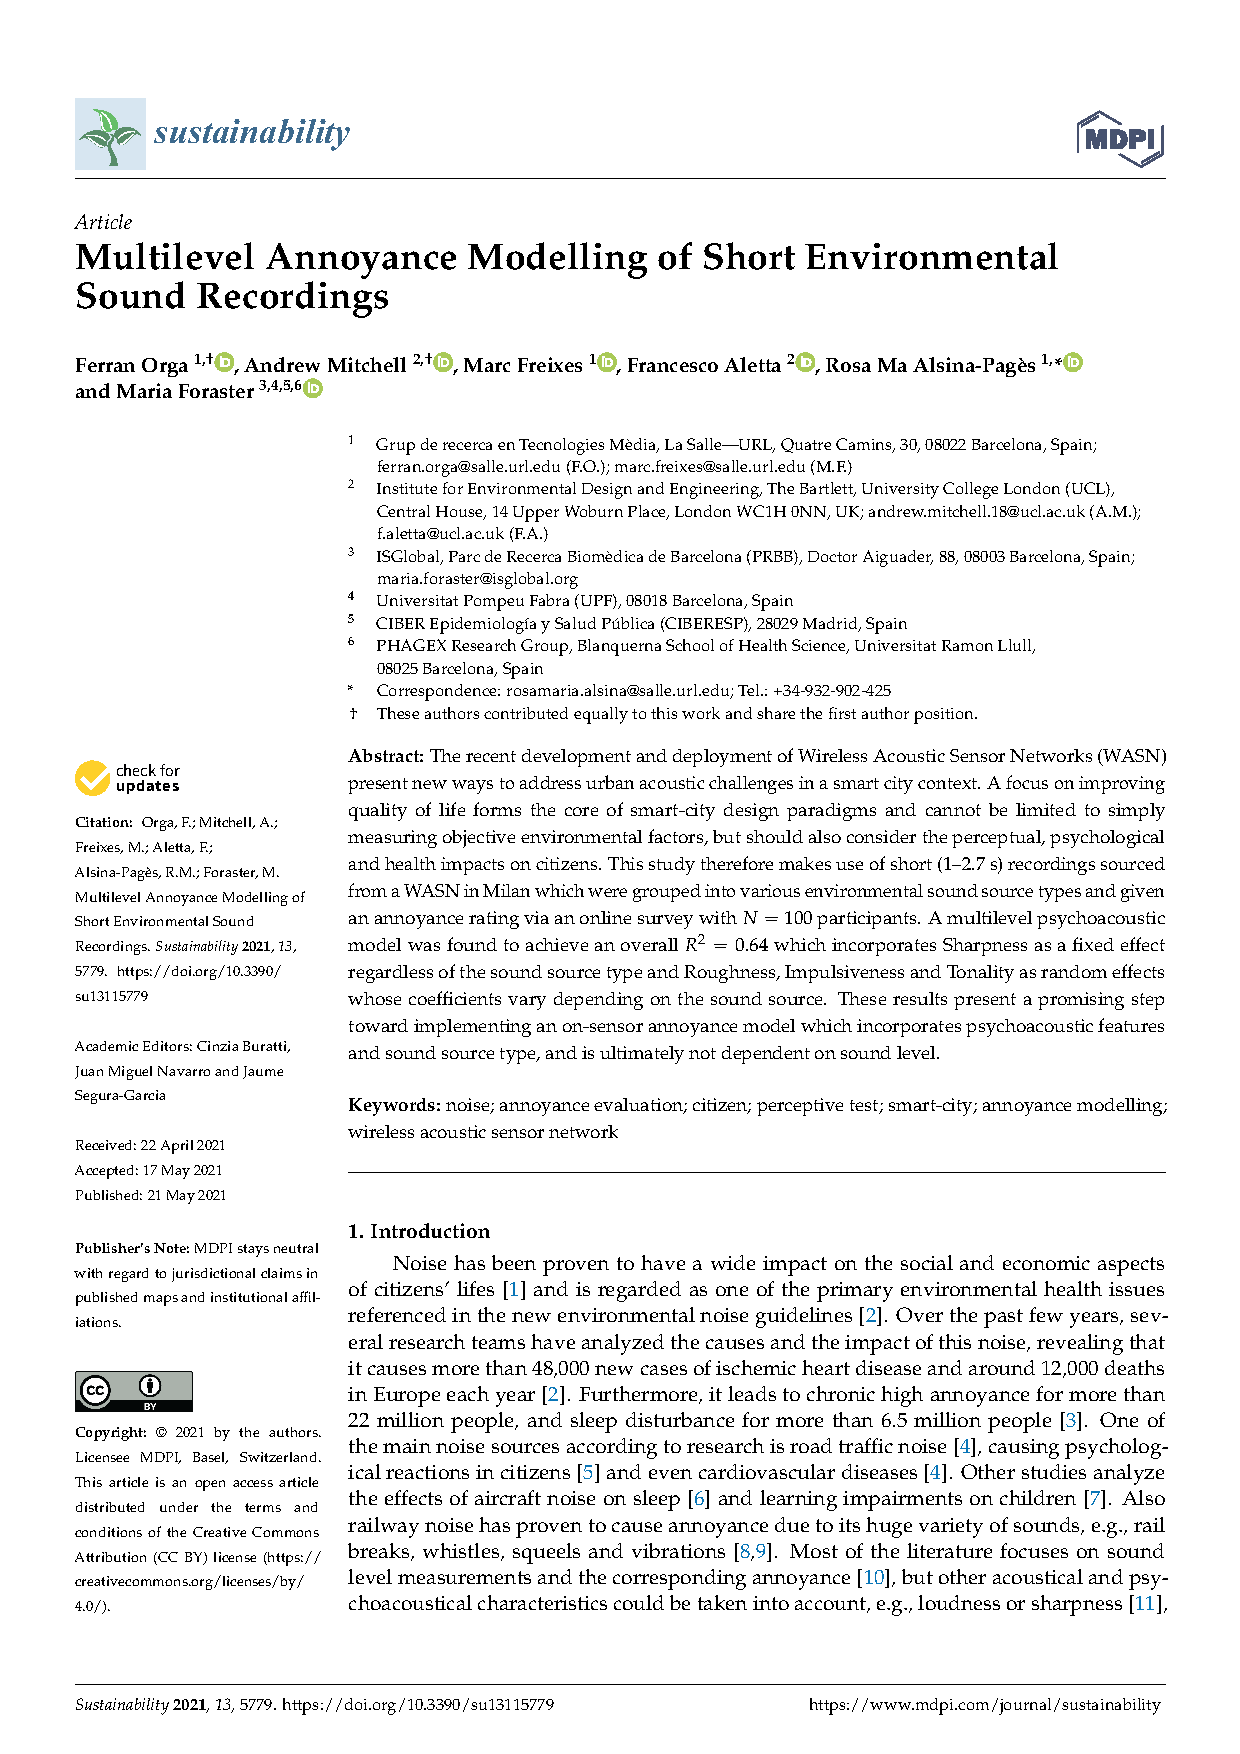
\includepdf[pages=-]{./Papers/Orga2021Multilevel.pdf}

%%%%%%%%%%%%%%%%%%%%%%%%%%%%%%%%%%%%%%%%%%%%%%%%%%%%%%%%%%%%%%%%%%%%%%%%%%%%%%%%%%%%%%%%%%%%%%%%%%%%

\section{Study III: Applied Predictive Soundscape Modelling: A Case Study Investigating Changes from the COVID-19 Lockdown}

\subsection*{Background and aims}
\hl{Some summary text here.}

\subsection*{Result and conclusion}

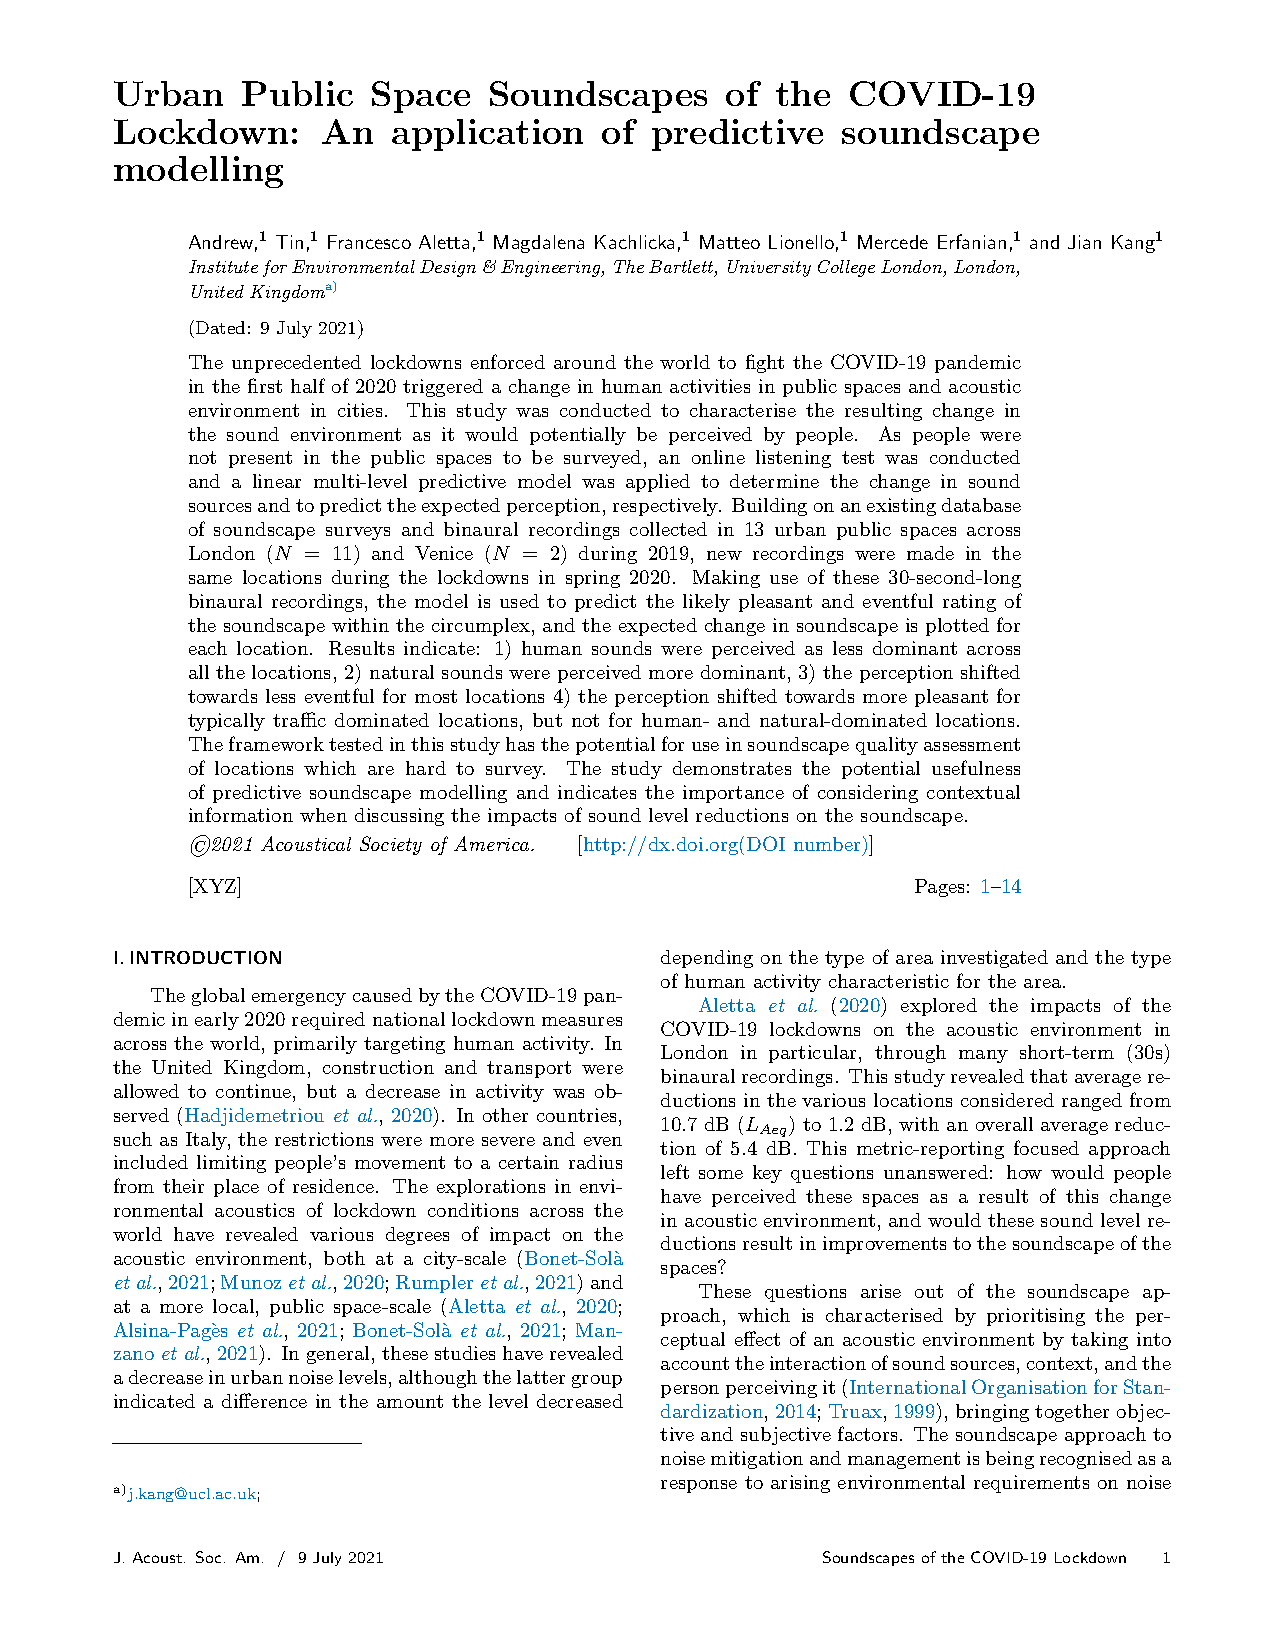
\includepdf[pages=-]{./Papers/Modelling_Lockdown_Soundscape_JASA.pdf}

%%%%%%%%%%%%%%%%%%%%%%%%%%%%%%%%%%%%%%%%%%%%%%%%%%%%%%%%%%%%%%%%%%%%%%%%%%%%%%%%%%%%%%%%%%%%%%%%%%%%


\newpage
\section{Study IV: A Temporal Convolutional Neural Network for Multi-label Sound Recognition and Annoyance Detection of Complex Soundscapes}

\subsection*{Background and aims}

\subsubsection*{Positivity (or the absence of negativity?)}
From the experience of the previous studies which are highly focused on the existing environmental acoustic and psychoacoustic metrics, one (of many) potential limitations has been revealed. For the most part, these metrics were designed to characterise various negative qualities of the sound. Certainly, they therefore have a negative correlation with positive assessments of the sound, but the simple fact is that they were conceived of and implemented in an attempt to quantify some sonic characteristic that was assumed by the researchers to contribute to a negative perception. Hence why in Zwicker's empirical formula for Psychoacoustic Annoyance \citep{PsychoacousticsfactsmodelsZwicker} $PA = N_5 (1 + \sqrt{\omega^2_S + \omega^2_{FR}})$, all of the constituent parts have positive coefficients.

While this would not theoretically hinder a formula for describing positive aspects of the sound, it creates a sort of conceptual barrier. If all of these metrics are designed to capture negative aspects of the sound, then it is insufficient to use them create a formula to describe a positive sound, since that formula would only represent the 'absence of negativity', not necessarily positivity.
\subsection*{Result and conclusion}

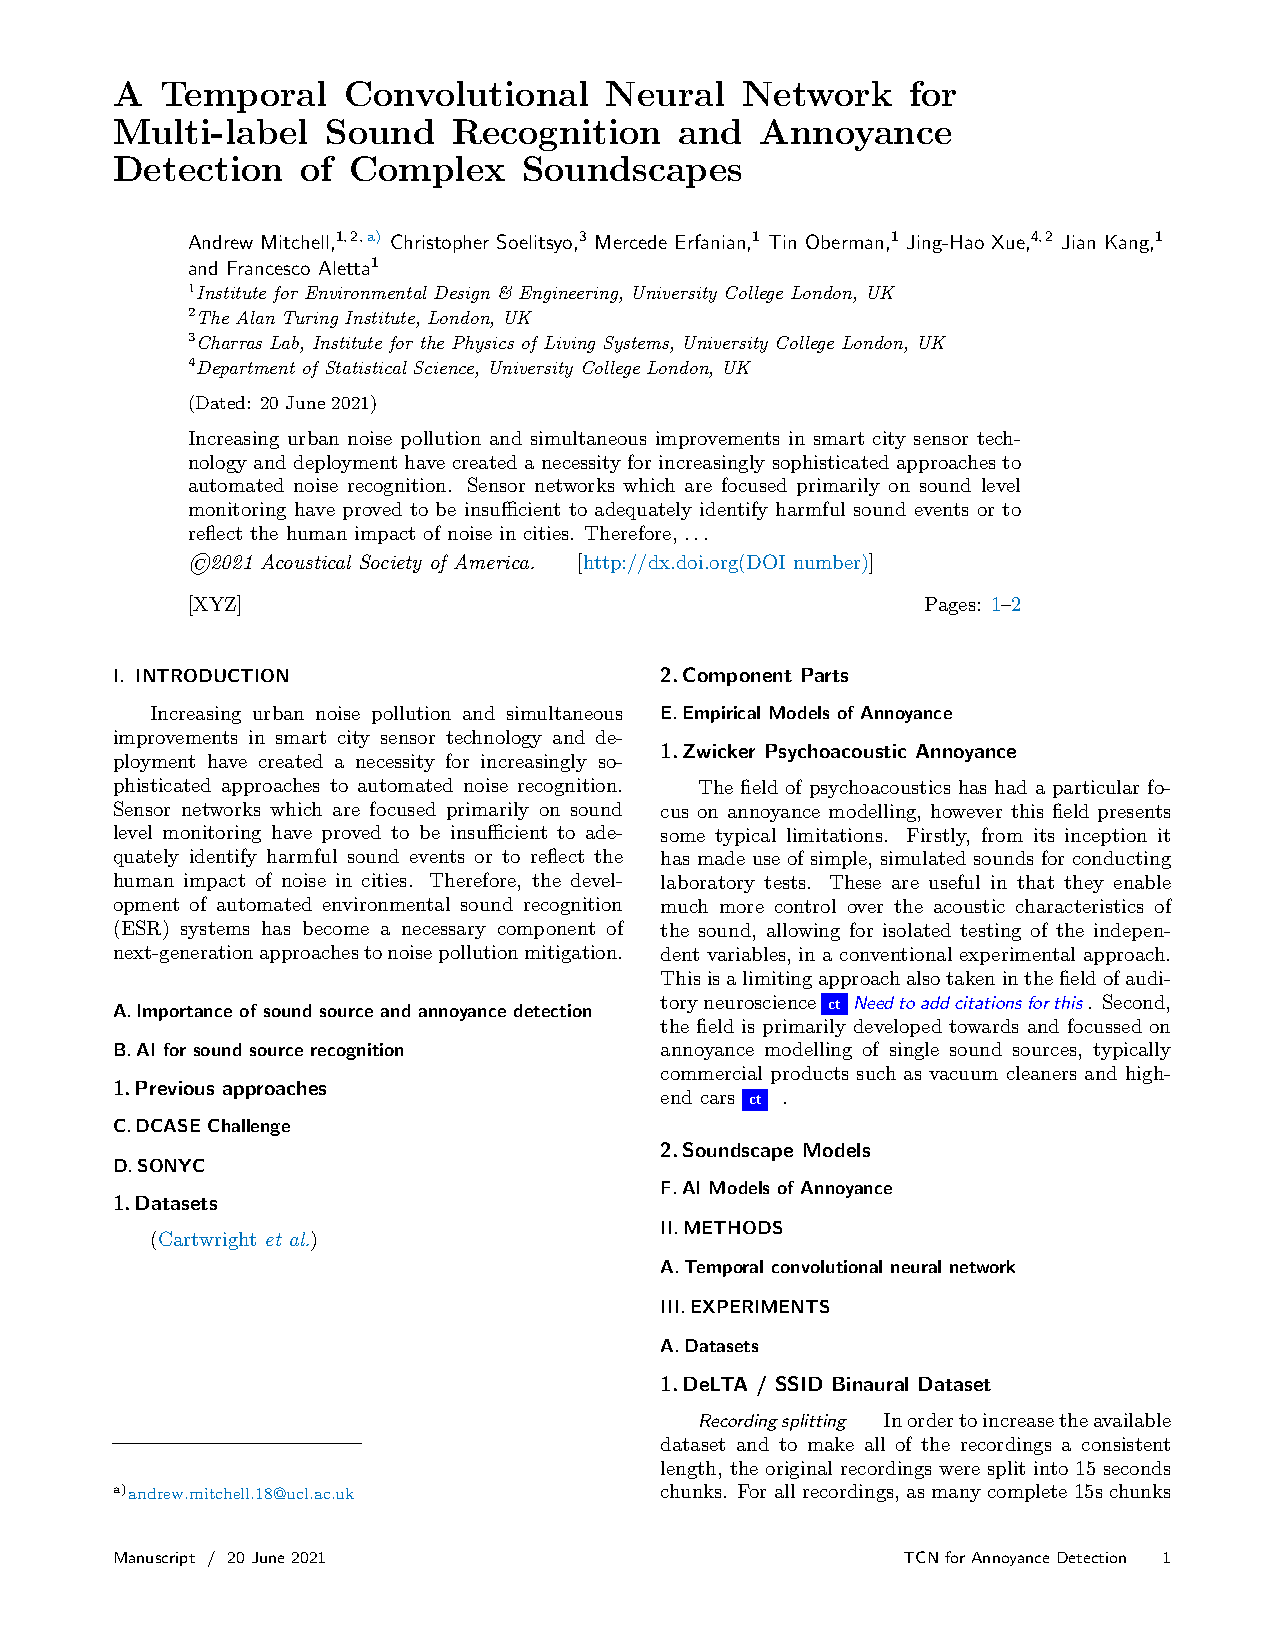
\includepdf[pages=-]{./Papers/IEEE_DeLTA_Preprint.pdf}

\section{Commentary: From Deterministic to Probabilistic Soundscapes: A critical tour around the soundscape circumplex}

\hl{Some summary text here.}

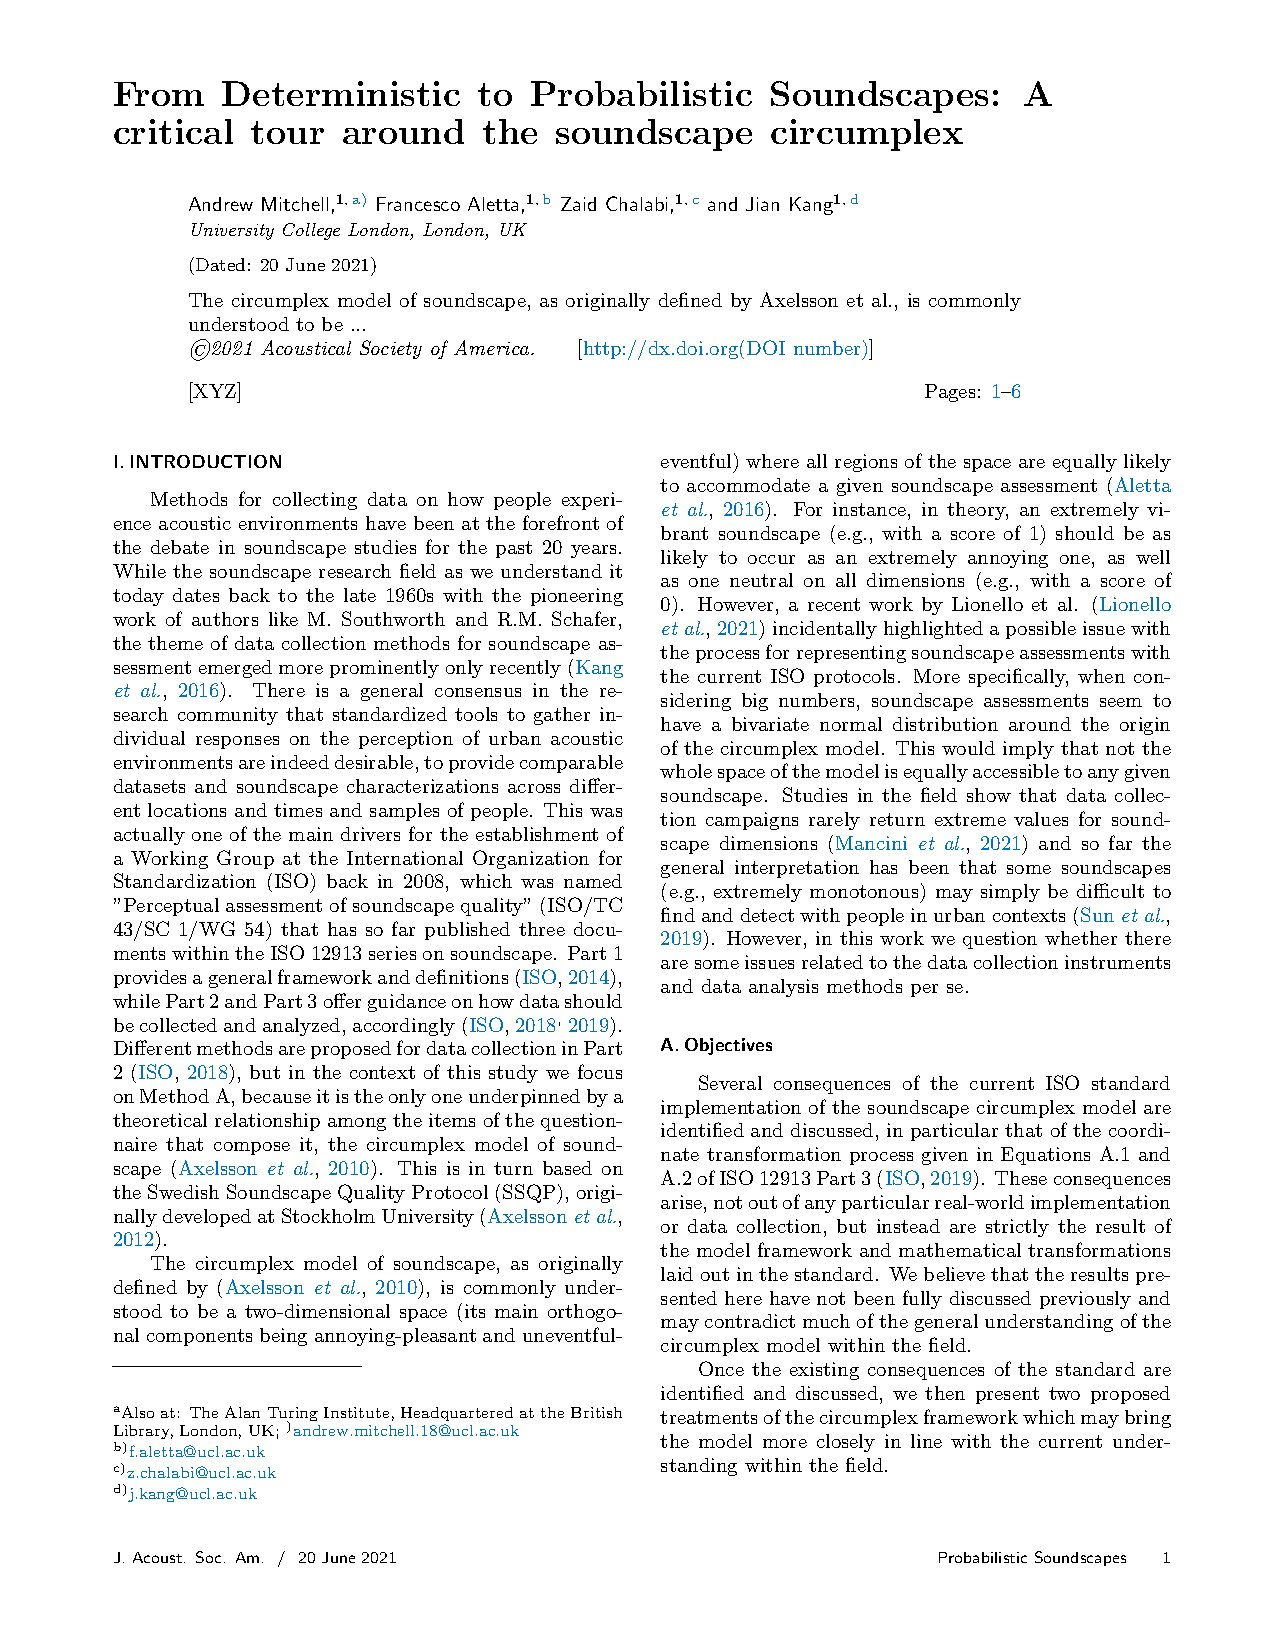
\includepdf[pages=-]{./Papers/J13_Circumplex_transform_Preprint.pdf}


%%%%%%%%%%%%%%%%%%%%%%%%%%%%%%%%%%%%%%%%%%%%%%%%%%%%%%%%%%%%%%%%%%%%%%%%%%%%%%%%%%%%%%%%%%%%%%%%%%

% \chapter{Introduction}
\label{ch:intro}

\section{Research Summary}
Urban noise pollution affects 80 million EU citizens with substantial impacts on public health which are not well addressed by conventional noise control methods. Traditional noise control methods have typically limited their focus to the reduction of unwanted noise, ignoring the potential benefits of increasing positive sounds and remaining restricted by practical limitations of noise reduction. Modern approaches to achieve improved health outcomes and public satisfaction aim to incorporate a person's perception of an acoustic environment, an approach known as 'Soundscape'.

Soundscape studies strive to understand the perception of a sound environment, in context, including acoustic, (non-acoustic) environmental, contextual, and personal factors. These factors combine together to form a person's soundscape in complex interacting ways \citep{Berglund2006Tool}. In order to predict how people would perceive an acoustic environment, it is essential to identify the underlying acoustic and non-acoustic properties of soundscape.

% From: Upgrade report
When attempting to apply soundscape in practical applications in the built environment, it is immediately apparent that a predictive model of the users' perceptual response to the acoustic environment is necessary. Whether to determine the impact of a design change, or to integrate a large scale data at neighbourhood and city levels, a mathematical model of the interacting factors will form a vital component of the implementation of the soundscape approach. This work is intended to identify methods for incorporating contextual and objective information into a useable and interpretable predictive model of urban soundscapes. In order to achieve this, a protocol for collecting the multi-level, multi-factor perceptual assessment data has been developed and implemented, resulting in a large soundscape database. Several avenues of investigation are then drawn from the database and addressed throughout this thesis. The primary research questions are:

% TODO: Try to move this to the end of the introduction.
\begin{enumerate}
  \item What are the primary acoustic features involved in soundscape formation and what are the driving interactions between acoustic features and soundscape assessment?
  \item How does the sound source composition in a complex sound environment mediate this interaction and how can this effect be simplified and modelled?
  \item How can the multiple levels of soundscape formation be simplified and integrated into a cohesive predictive model, and what interpretations about the cross-effects of these levels can be drawn from the model?
  \item In what ways and to what extent can predictive soundscape modelling be applied to address future urban design challenges? How can these methods best be integrated into policy, design, noise mapping, and engineering practice?
\end{enumerate}

Towards answering these questions, the results of five %TODO: check this number at the end.
peer-reviewed studies are presented. These studies represent a series of work to 

\begin{enumerate}
  \item Advance the conceptual development and practice of soundscape studies
  \item Develop a transparent and useful method of predicting soundscape assessments
  \item Investigate the various components which influence soundscape perception, including personal factors like psychological well-being, acoustical factors, and sound source specifics and to integrate these components into the predictive modelling methods.
\end{enumerate}

\section{The SSID Project}
The \gls{ssid} Project is a five-year, multi-disciplinary project funded by a Horizon 2020 European Research Council grant (no. 740696).

\subsection{Project collaborators}

\subsection{Motivation for the SSID Project}

\section{Research Aims}

\section{Soundscape Indices and Metrics}

\section{General Aim}

% \chapter{Literature Review}
\label{ch:lit}

\section{Impact of Urban Noise on Health and Wellbeing}

\cit{Environmental noise in Europe 2020}

\hl{Give a full formal background to why noise control is important for public health}.
% https://www.euro.who.int/__data/assets/pdf_file/0008/383921/noise-guidelines-eng.pdf?ua=1

\section{Current Methods of Assessing and Addressing Urban Noise}

The approach to a practical predictive soundscape model arrived at within this thesis is heavily based on past environmental acoustics approaches. I will therefore begin with a brief summary of these past approaches.

\subsection{Acoustical Parameters}

\subsection{ISO Environmental Acoustics Standards}
\hl{ISO 1996-1, esp sections on annoyance, e.g. Annex F, G, H}

\subsection{EU Noise Mapping}

\cit{Environmental noise in Europe 2020}

\subsection{Shortcomings}


\section{Soundscape Studies}

\subsection{Soundscape Descriptors and Indices}

\subsection{World Soundscape Project}

\subsection{Swedish Soundscape Quality Protocol}


\subsection{Demographic differences}
Several studies have attempted to study the degree to which personal and demographic factors influence a person's soundscape perception. In some conceptions \cit{Kou2020effects} % CITE add Erfanian 2020
these personal factors are classed as 'contextual' soundscape indicators - features which influence or, in a modelling context, be used as independent variables to predict the value of a soundscape descriptor. The personal factors help to create a personal soundscape interpretation model which is individual to each person.

In this way, a person's individual state-of-mind, ethnic identity, educational background, gender identity, etc. form a pseudo-deterministic framework %! what a load of crap
through which the physical inputs from their environment are filtered. Clearly, many of these personal factors could never be measured and even those which are measurable will have wide ranges of legitimate effects, however estimating the degree and type of effect they may have can both help us better predict individual soundscape assessments and understand how group identities influence sound perception.

%TODO: Need to include earlier, more foundational studies into demographic factors

\paragraph*{Section on Erfanian et al. 2020, Psychological Well-being}

\paragraph*{Low-income and minority evidence} % FIXME I think this section will need to be heavily revised for phrasing and content. I'm not happy with how I'm discussing under-represented groups.
A consistent limitation of soundscape studies investigating the influence of personal factors is a sampling bias towards majority ethnicities (typically White British for UK studies and ethnic Chinese for Chinese studies) and middle-class and highly educated groups. % CITE Hoo boy citation definitely needed
This results in not only incomplete information about how demographics influence soundscape perception, but also represents a systemic under-representation of certain environments. While it may be unclear to what extent ethnicity and social class internally influence a person's perception, it is clear that these groups are exposed to different sound environments % NOTE: socio-economic studies - Huan 2019? Jian ~2015?, Environmental noise in Europe 2020

and therefore studies which do not include under-represented groups are also by definition not including those sound environments which those groups inhabit.

A recent study by \cit{Kou2020effects} was successful in making inroads in these under-represented environments by studying the Humboldt Park neighbourhood in Chicago, USA. Their study included
% TODO: Finish summarising results from Kou2020


\section{Approaches to Soundscape in Engineering}

From this literature review, some conclusions about current approaches to incorporating the concept of "soundscape" into practical engineering and architectural design have been identified.

\subsection{The Quiet Areas approach}

This approach maintains a focus on "identifying and preserving quiet areas" \cit{Environmental noise in Europe 2020} following the imperative given in the Environmental Noise Directive \cit{END}. This approach is mostly rooted in a noise mindset, although the methods employed for identifying quiet areas varies across countries within the EEA. Background sound levels seem to play an important role in identifying quiet areas, in particular when attempting to

%TODO Continue adding from Remarkable notes

\section{Existing Predictive Models}

Contrary to the hopes expressed by \citet{Aletta2014Towards}, that "ideally there should be one acoustic indicator per dimension", the evidence from subsequent investigations and modelling attempts \citep{Lionello2020systematic} indicates this to be unlikely. There appears to be no reason we should think the perceptual dimensions should be reduced to a single acoustic indicator. The dimensions of soundscape represent complex perceptual concepts which we should expect to be composed of a multi-factor interaction between the input features. This necessary complexity  highlights the need for a more sophisticated machine learning approach in order to handle and interpret the interactions between the many input features which contribute to the formation of a soundscape perception.
\citep{Aletta2016Soundscape}

\citep{Lionello2020systematic}

\subsection{Models based on non-acoustic data sources}

\citep{Verma2020Predicting}, \citep{Gasco2020Social}

% \chapter{Methods}
\label{chap:methods}

%%%%%%%%%%%%%%%%%%%%%%%%%%%%%
%FIXME: Find a better spot for this
The ability to predict the likely soundscape assessment of a space is crucial to implementing the soundscape concept in practical design. Current methods of assessing soundscapes are generally limited to a post-hoc assessment of the existing environment, where users of the space in question are surveyed regarding their experience of the acoustic environment \citep{Engel2018Review, Zhang2018Effect}. While this approach has proved useful in identifying the impacts of an existing environment, designers require the ability to predict how a change or proposed design will impact the soundscape of the space. To this end, a model that is built upon measurable or estimate-able quantities of the environment would represent a leap forward in the ability to design soundscapes.

\section{Questionnaires}

 The full protocol developed for this thesis is outlined in Chapter \ref{chap:protocol}. The development and presentation of this protocol involved a substantial development and testing phase, and represents a novel advancement in soundscape survey methodology. Therefore it was submitted and published as a peer-reviewed journal article in MDPI Applied Sciences as \citet{Mitchell2020Soundscape} and is presented as a stand-alone chapter within this thesis.

 \subsection{Likert Responses}

 \subsection{Circumplex Projection}

\section{Psychoacoustics and Auditory Perception}

 \subsection{Psychoacoustic Parameters}

   \subsubsection{Loudness}
   \emph{Zwicker and Fastl, Chap 8, see Mendeley notes and python-acoustics development notes.}
 \subsection{Feature Selection}

\section{Machine Learning and Regression Techniques}

 \subsection{Feature Selection}
   \subsubsection{Mutual Information}
   \draft{It appears that mutual information is related to the Bayes formula. I still need to read more into this, but it appears based on relative and overlapping probability distributions between the variables in question.}
   \paragraph*{From scholarpedia:}
   % http://www.scholarpedia.org/article/Mutual_information
   \draft{Based on entropy, where the uncertainty about a variable can be expressed as "the number of yes/no questions it takes to guess a random variable, given knowledge of the underlying distribution and taking the optimal question-asking strategy". "The mutual information is therefore the \emph{reduction} in uncertainty about variable $X$, or the expected reduction in the number of yes/no questions needed to guess $X$ after observing $Y$.". }

   \draft{"Mutual Information is just one way among many of measuring how related two variables are. However, it is a measure ideally suited for analyzing communication channels. Abstractly, a communication channel can be visualized as a transmission medium which receives an input $x$ and produces an output $y$. If the channel is \emph{noiseless}, the output will be equal to the input. However, in general, the transmission medium is noisy and an input $x$ is converted to an output $y$ with probability $P_{Y|X}(y|x)$. }
   \misc{This seems very useful for my conception of sound perception / auditory processing, where the perception system is a noisy communication channel.}

   \subsubsection{Conditional Mutual Information}
   The Mutual Information between two variables, given another variable as a control.

 \subsection{Clustering Analysis}
   \paragraph{K-means}
   \paragraph{nbclust}

 \subsection{Modelling Likert-type Data}

   \subsubsection{Multiple Linear Regression}

   \subsubsection{Ordinal Logistic Regression}

   \subsubsection{Multi-output Regression}

 \subsection{Multi-level Models}

 \subsection{Bayesian Regression}


% \chapter{Characterizing the Temporal Behaviour of Dynamic Urban Soundscapes}
\label{ch:temp}

\section{Introduction}

\section{Methods}

\section{Results and Discussion}
  \subsection{Presence of 1/f in urban soundscapes}
  \subsection{Statistical relationship to pleasantness ratings}
  \subsection{Ordinal logistic models based on temporal and acoustic features}

\section{Conclusion}

% \chapter{Combined Multi-level Regression Model for Predicting Soundscape}
\label{ch:mlm}

\section{Introduction}

\section{Methods}
  \subsection{Multi-level regression modelling}
  \subsection{Feature Selection}

\section{Results}
  \subsection{Simplified predictive soundscape models}
    \paragraph*{COVID-19 Model}

  \subsection{Multiple levels of soundscape formation}

  \subsection{Feature selection}
    \paragraph*{Acoustic features}
    \paragraph*{Non-acoustic factors}

  \subsection{Model design}

\section{Discussion}
  \subsection{Interpretation}
  \subsection{Implementation and use cases}



% \chapter{The Influence of Sound Source Composition in Soundscape Formation}
\label{ch:ssp}

\section{Introduction}

\section{Methods}
  \subsection{Data collection}
  \subsection{Clustering analysis}

\section{Results}
  \subsection{Sound source profiles}
  \subsection{Perceived affective quality ratings}
  \subsection{Psychological well-being mediates soundscape formation within different sound source profiles}
  \subsection{Regression models}

\section{Discussion}

\section{Conclusion}


% \chapter{A Bayesian Hierarchical Predictive Soundscape Model and a Proposed Soundscape Index}
\label{ch:bayes}

\section{Introduction}

\section{Methods}

\section{Results}

\section{Discussion}

\section{Communicating SSID on the Basis of Percentages}

\section{Conclusion}


% \chapter{Soundscape Modelling for Smart Cities: A case study}
\label{ch:smart}

\section{Introduction}

\section{Methods}
  \subsection{SSID Data Collection}
  \subsection{Sensor network and IFSTTAR data collection}

\section{Results}

\section{Discussion}



\chapter{Conclusions}
\label{ch:conc}

\section{General Discussion}

\section{Developing a framework for sustainable soundscapes}

\subsection{Defining Sustainability}



\section{Implications}

\section{Limitations and Recommendations for Future Research}

\section{Concluding Remarks}


%%%%%%%%%%%%%%%%%%%%%%%%%%%%%%%%%%%%%%%%%%%%%%%%%%%%%%%%%%%%%%%%%%%%%%%%%%%%%%%%%%%%%%%%%%%%%%%%%%


\backmatter
% A glossary and list of acronyms may go here
% or may go in the front matter after the abstract.
\printglossaries

% The bibliography will go here.
\bibliography{thesis_refs}

%%%%%%%%%%%%%%%%%%%%%%%%%%%%%%%%%%%%%%%%%%%%%%%%%%%%%%%%%%%%%%%%%%%%%%%%%%%%%%%%%%%%%%%%%%%%%%%%%%

\end{document}
